\documentclass{article}


\usepackage[round]{natbib}
\usepackage{amsmath,amssymb,amsthm,bm,enumerate,mathrsfs,mathtools}
\usepackage{latexsym,color,verbatim,multirow}
\usepackage{graphicx}
\usepackage{caption}
\usepackage{subcaption}
\usepackage{tikz}
\usepackage{geometry}
\usetikzlibrary{shapes,arrows}
\tikzstyle{block} = [rectangle, draw, fill=white!20,
    text width=7em, text centered, rounded corners, minimum height=4em]
\tikzstyle{title} = [text width=7em, text centered, font=\bfseries]
\tikzstyle{line} = [draw, -latex']


\usepackage{mycommands}

\begin{document}

\newtheorem{theorem}{Theorem}
\newtheorem{corollary}[theorem]{Corollary}
\newtheorem{lemma}[theorem]{Lemma}
\newtheorem{observation}[theorem]{Observation}
\newtheorem{proposition}[theorem]{Proposition}
\newtheorem{definition}[theorem]{Definition}
\newtheorem{claim}[theorem]{Claim}
\newtheorem{fact}[theorem]{Fact}
\newtheorem{assumption}[theorem]{Assumption}
\newtheorem{model}[theorem]{Model}

\theoremstyle{definition}
\newtheorem{example}{Example}

\newcommand{\cM}{\mathcal{M}}
\newcommand{\cH}{\mathcal{H}}
\newcommand{\cD}{\mathcal{D}}
\newcommand{\FDR}{\textnormal{FDR}}
\newcommand{\FCR}{\textnormal{FCR}}
\newcommand{\crt}{\phi}
\newcommand{\M}{\mathcal{M}}
\newcommand{\cY}{\mathcal{Y}}
\newcommand{\cX}{\mathcal{X}}
\newcommand{\cV}{\mathcal{V}}
\newcommand{\bX}{\mathbf{X}}
\newcommand{\x}{\mathbf{x}}
\newcommand{\Gv}{\;\;\big|\;\;}
%\newcommand{\cP}{\mathcal{P}}
\newcommand{\proj}{\cP}
\newcommand{\pow}{\text{Pow}}
\newcommand{\sF}{\mathscr{F}}
\newcommand{\cF}{\mathcal{F}}
\newcommand{\sC}{\mathscr{C}}
\newcommand{\hJ}{\widehat{J}}
\newcommand{\bH}{\mathbf{H}}
\newcommand{\bM}{\mathbf{M}}
\newcommand{\tM}{\widetilde{M}}
\newcommand{\tE}{\widetilde{E}}
\newcommand{\tV}{\widetilde{V}}
\newcommand{\tR}{\widetilde{R}}
\newcommand{\tL}{\widetilde{L}}
\newcommand{\hk}{\hat{k}}
\newcommand{\hr}{\hat{r}}       
\newcommand{\cN}{\mathcal{N}}
\newcommand{\cJ}{\mathcal{J}}
\newcommand{\leqAS}{\overset{\textrm{a.s.}}{\leq}}
\newcommand{\Err}{\mathcal{E}}
\newcommand{\RSS}{\text{RSS}}


\newcommand*\mystrut{\vrule width0pt height0pt depth1.5ex\relax}
\newcommand{\underlabel}{\underbracket[1pt][.5pt]{\mystrut \quad\;\; \sub \quad\;\; }}
\newcommand{\JTcomment}[1]{{\color{blue}{(JT: \bf \sc #1) }}}
\newcommand{\WFcomment}[1]{{\color{red}{(WF: \bf \sc #1) }}}
\newcommand{\RTcomment}[1]{{\color{green}{(RT: \bf \sc #1) }}}

\title{Selective Sequential Model Selection}
\author{William Fithian, Jonathan Taylor, Rob Tibshirani, and Ryan Tibshirani}
\maketitle

\begin{abstract}
  Many model selection algorithms produce a path of fits specifying a sequence of increasingly complex models. Given such a sequence and the data used to produce them, we consider the problem of choosing the least complex model that is not falsified by the data. Extending the selected-model tests of \citet{fithian2014optimal}, we construct $p$-values for each step in the path, accounting for the fact that the model path is determined adaptively using the data. In the case of linear regression, our $p$-values improve on the power of the spacings test of \citet{taylor2014exact}, sometimes dramatically.

To select a model, we can feed the resulting $p$-values as inputs into sequential stopping rules such as those proposed by \citet{gsell2013sequential} and \citet{li2015accumulation}, achieving control of the familywise error rate or false discovery rate as desired. Some stopping rules require the null $p$-values to be independent of each other and of the non-null $p$-values, a condition not satisfied by the saturated-model $p$-values of \citet{taylor2014exact}. We derive intuitive and general conditions for independence and show that our proposed constructions yield independent $p$-values. We also discuss connections between the selected-model test and parametric bootstrap sampling.
\end{abstract}

\section{Introduction}
\label{sec:introduction}
Many model selection procedures produce a sequence of increasingly complex models, leaving the data analyst to choose among them. 
%While methods like cross-validation aim at minimizing out-of-sample prediction error, such methods tend to select a large fraction of noise variables. 
Given such a path, we consider the problem of choosing the simplest model in the path that is not falsified by the available data. Examples of path algorithms include forward stepwise linear regression, least angle regression (LAR) and  the ever-active path in $\ell_1$-regularized models. \citet{taylor2014exact} study methods for generating exact $p$-values at each step of these path algorithms, and their methods provide a starting point for our proposals. In addition, \citet{choi2014selecting} discuss a selective approach to determining the correct rank of the covariance matrix in principle components analysis.



To select a model, we compute a set of sequential $p$-values at each step of the model path, and then feed them into a stopping rule that is guaranteed to control the FDR, familywise error rate (FWER), or a similar quantity. Recently \citet{gsell2013sequential} and \citet{li2015accumulation} proposed sequential stopping rules of this kind. 
Both sets of rules require that once we have reached the first correct model in our path, the $p$-values in subsequent steps are uniform (or conservative),
and independent. In this paper we develop a theoretical framework for constructing sequential $p$-values that are both uniform and independent under the correct model, and show how to construct them in forward stepwise regression, LAR and the ever-active path in $\ell_1$-regularized models. 

While our approach and analysis are quite general, we begin by introducing a specific example: the selective max-$t$ test for forward stepwise regression, a selective sequential version of the max-$t$ test of \citet{buja2014}, generalized using the theory in \citet{fithian2014optimal}.

\subsection{The max-$t$ Test in Forward Stepwise Regression}

Forward stepwise regression is a greedy algorithm for building a sequence of nested linear regression models. At each iteration, it augments the current model by including the variable that will minimize the residual sum of squares of the next fitted model. Equivalently, it selects the variable with the largest $t$-statistic, controlling for the variables in the current model.

Let $E \sub \{1, \ldots, d\}$ denote the current {\em active set}, the set of predictor variables already selected, and let $\RSS(E)$ denote the residual sum of squares for the corresponding regression model. For $j\notin E$ let $t_{j,E}(Y)$ denote the multivariate $t$-statistic of variable $j$, adjusting for the active variables. Using the standard result that
\begin{equation}
t_{j,E}^2 = (n-|E|-1) \frac{\RSS(E) - \RSS(E \cup \{j\})}{\RSS(E \cup \{j\})},
\end{equation}
we see that the next variable selected is 
\begin{equation}
j^* = \argmax_{j\notin E} |t_{j,E}| = \argmin_{j\notin E} \RSS(E \cup \{j\}),
\end{equation}
with corresponding $t$-statistic $t_E^* = t_{j^*,E}$. The selective max-$t$ test rejects for large values of $t_E^*$, compared to an appropriate conditional distribution that accounts for the adaptive selection of the model path.

Table~\ref{tab:diab} illustrates the max-$t$ test and two others applied to the diabetes data from \cite{LARS}, consisting of observations of $n=442$ patients. The response of interest is a quantitative measure of disease progression one year after baseline, and there are ten measured predictors --- age, sex, body-mass index, average blood pressure, and six blood serum measurements --- plus quadratic terms, giving a total of $d=64$ features. We apply forward stepwise regression to generate the model path (beginning with an intercept term), and then use each of the three methods to generate $p$-values at each step along the path. Finally, we use the ForwardStop rule \citep{gsell2013sequential} at FDR level $\alpha=0.1$ to select a model based on the sequence of $p$-values. The red entry in each column indicates the last variable selected by ForwardStop.

\begin{table}[ht]
\centering
\begin{tabular}{|l|c|c|c|c|c|}
\hline
 Step & Variable &  Nominal pvalue &  Saturated pvalue &  MaxT pvalue \\
\hline
    1 &      bmi &            0.00 &              0.00 &         0.00 \\
    2 &      ltg &            0.00 &              0.00 &         0.00 \\
    3 &      map &            0.00 &             {\color{red} 0.05} &         0.00 \\
    4 &  age:sex &            0.00 &              0.33 &         0.02 \\
    5 &  bmi:map &            0.00 &              0.76 &         0.08 \\
    6 &      hdl &            0.00 &              0.25 &         0.06 \\
    7 &      sex &            0.00 &              0.00 &         0.00 \\
    8 &    glu$^2$ &            0.02 &              0.03 &         {\color{red} 0.32} \\
    9 &    age$^2$ &            0.11 &              0.55 &         0.94 \\
   10 &  map:glu &            0.17 &              0.91 &         0.91 \\
   11 &       tc &            0.15 &              0.37 &         0.25 \\
   12 &      ldl &            0.06 &              0.15 &         0.01 \\
   13 &    ltg$^2$ &            0.00 &              0.07 &         0.04 \\
   14 &  age:ldl &            0.19 &              0.97 &         0.85 \\
   15 &   age:tc &            0.08 &              0.15 &         0.03 \\
   16 &  sex:map &            0.18 &              0.05 &         0.40 \\
   17 &      glu &            0.23 &              0.45 &         0.58 \\
   18 &      tch &       {\color{red}     0.31} &              0.71 &         0.82 \\
   19 &  sex:tch &            0.22 &              0.40 &         0.51 \\
   20 &  sex:bmi &            0.27 &              0.60 &         0.44 \\
\hline
\end{tabular}


\caption[tab:diab]{\em Forward stepwise regression for the diabetes data: naive $p$-values, $p$-values from the saturated model, and our max-$t$ $p$-values. The red annotation indicates the model selected by ForwardStop with $\alpha=0.1$. For the max-$t$ $p$-values, this stopping rule gives exact $\text{FDR}_{\text{model}}$ control at the 10\% level.}
\label{tab:diab}
\end{table}

The nominal $p$-values in Table~\ref{tab:diab} are computed by comparing $t_E^*$ to the $t_{n-|E|-1}$-distribution, which would be the correct distribution if the sequence of models were selected ahead of time, before observing the data. Because the model sequence is in fact selected adaptively to maximize the value of $t_E^*$, this method is highly anti-conservative.

The max-$t$ test $p$-values are computed using the same test statistic $|t_E^*|$, but compared with a more appropriate null distribution. We can simulate the distribution of $|t_E^*|$ under the null model, i.e. the linear regression model specified by active set $E$:
\begin{equation}
  M(E):\; Y \sim N(X_E\beta, \sigma^2 I), \quad \beta\in \R^{|E|}, \sigma^2>0,
\end{equation}
where $X_E$ is the matrix with columns $(X_j)_{j\in E}$. Because $U_E=\left(X_E'Y,\, \|Y\|^2\right)$ is the complete sufficient statistic for $M(E)$, we can sample from the conditional null distribution of $t_E^*$ given $U_E$ and the current active set $E$, using the {\em selected-model test} framework of \citet{fithian2014optimal}. In step one, because $E=\{1_n\}$ is fixed and $t_E^*$ is independent of $U_E$, the conditional test reduces to the max-$t$ test proposed in \citet{buja2014}. In later steps, $t_E^*$ and $U_E$ are not conditionally independent of $E$, but we can estimate the null conditional distribution through Monte Carlo sampling.

The saturated-model $p$-values also account for selection, but they rely on somewhat different assumptions, condition on more information, and test a slightly less restrictive null hypothesis. We discuss these distinctions in detail in Section~\ref{sec:whichnull}.

For most of the early steps in Table~\ref{tab:diab}, the (invalid) nominal test gives the smallest $p$-values, followed by the max-$t$ test, then the saturated-model test. Both the max-$t$ and saturated-model $p$-values are exactly uniform under the null, but the max-$t$ $p$-values appear to be more powerful under the alternative. As we will discuss in Section~\ref{sec:selective-reg}, selected-model tests such as the max-$t$ can be much more powerful than saturated-model tests in early steps of the path when multiple strong variables are compete with each other to enter the model first. Using the max-$t$ $p$-values, ForwardStop selects a model of size 8, compared to size 3 when using the saturated-model $p$-values. 

Because the max-$t$ null $p$-values are independent, while the saturated-model $p$-values are not, ForwardStop is guaranteed to control FDR when using the former but not the latter. In Section~\ref{sec:pValsIndep} we discuss intuitive sufficient conditions for independence and show that the max-$t$ and many other selected-model tests satisfy these conditions.

\begin{comment}
The latter two sets of $p$-values test somewhat different hypotheses:  the $p$-values from the saturated model test whether the partial regression of the predictor just added is zero after regressing out the variables already in the model, what we call the ``incremental null''
In contrast, the max-$t$ $p$-values test whether the current model is adequate; that is, whether all predictors not in the model  have coefficients equal to zero, the ``complete null''. (The issue of what hypothesis to test is discussed in section \ref{sec:whichnull}.)
\end{comment}


\subsection{Outline}

For the remainder of the article we will discuss the problem of selective sequential model selection in some generality, returning periodically to the selective max-$t$ test in forward stepwise regression and its lasso regression counterpart, the next-$\lambda$ test, as intuitive and practically important running examples. 

In comparison to their saturated-model counterparts, we will see that the selected-model tests proposed here have three main advantages: power, independence (in some cases), and generalizability beyond linear regression. These advantages do not come entirely for free, as we will see: the selected-model methods test a more restrictive null hypothesis than the saturated-model methods. In addition, the selected-model test require accept-reject or MCMC sampling, while the saturated-model tests are available in closed form.

Section~\ref{sec:genericSetting} introduces the general problem setting, gives important definitions, and reviews relevant literature on testing ordered hypotheses using a sequence of $p$-values. Many of these methods require the $p$-values to be uniform and independent under the null, and we derive general conditions to ensure this property in Section~\ref{sec:pValsIndep}. In Section~\ref{sec:selective-reg} we contrast selected-model and saturated-model tests for linear regression setting, and illustrate why selected-model tests are often much more powerful in early steps of the path. In Section~\ref{sec:computation} we discuss strategies for sampling from the null distribution for our tests, and prove that in forward stepwise regression and $\ell_1$-regularized likelihood methods, the number of constraints in the sampling problem is never more than twice the number of variables. We provide a simulation study in Section~\ref{sec:sparseReg} and briefly discuss applications of our framework to principal components analysis in Section~\ref{sec:pca}. The paper ends with a Discussion.

\section{Selective Sequential Model Selection}
\label{sec:genericSetting}

In the general setting, we observe data $Y \in \cY$ with unknown sampling distribution $F$, and then apply some algorithm to generate an adaptive sequence of $d$ nested statistical models contained in some {\em upper model} $M_{\infty}$.
\[
M_0(Y) \sub M_1(Y) \sub \cdots \sub M_d(Y) \sub M_\infty.
\]
By {\em model}, we mean a family of candidate probability distributions for $Y$. For example in  linear regression, a model specifies  the set of
predictors with nonzero coefficients (but not the  values of their coefficients). Without loss of generality, we can take $M_\infty$ as the union of all models under consideration. We will use the notation $M_{0:d}$ to denote the sequence $M_0, \ldots, M_d$, which we call the {\em model path}. We assume throughout that for each candidate model $M$ there is a minimal sufficient statistic $U(Y; \,M)$, and write
\[
U_k(Y) = U(Y; \,M_k(Y)).
\]

Given data $Y$ and model path $M_{0:d}$, we set ourselves the formal goal of selecting the simplest correct model: the smallest $k$ for which $F\in M_k(Y)$. Of course, in most real data problems all of the $M_k(Y)$, as well as all other models under consideration, are incorrect. In more informal terms, then, we seek the simplest model in the path that is not refuted by the available data.

\JTcomment{ Not sure if stopping rule is a great name. It suggests it is a ``stopping time'' with respect to some filtration (which it often is). But it doesn't have to be. Or maybe we should say we call it stopping because we use the property of it being a stopping time? 

Another notation quibble for $M(E)$ I kind of prefer the notation $(\beta_E, \sigma^2_E)$ instead of $(\beta, \sigma^2)$. It emphasizes that these are parameters of different models.}

Define the {\em completion index} $k_0(Y) = \min\{k:\; F \in M_k(Y)\}$, the index of the first correct model. By construction, $F\in M_k \iff k \geq k_0$. A {\em stopping rule} is any estimator $\hk(Y)$ of $k_0$, with $M_k$ ``rejected'' if $k < \hk$, and ``accepted'' otherwise. Because $\hk$ is the number of models we do reject, and $k_0$ is the number we should reject, the number of type I errors is $V=(\hk-k_0)_+$, while the number of type II errors is $(k_0-\hk)_+$. Depending on the scientific context, we might want to control the familywise error rate (FWER) $\P(V>0)$, the false discovery rate (FDR) $\E[V/\hk; \hk>0]$ \citep{benjamini1995controlling}, or another error rate defined by the expectation of some loss function $g(\hk, k_0)$:
\begin{equation}\label{eq:errRate}
\Err_F(\hk(\cdot), g) = \E_F\left[ g\left(\hk(Y), k_0(Y)\right)\right]
\end{equation}

\subsection{Single-Step $p$-Values}

We will restrict our attention to stopping rules like those recently proposed by \citet{gsell2013sequential} and \citet{li2015accumulation}, which operate on a sequence $p_{1:d}$ of $p$-values. At each step $k$, we will construct a $p$-value for testing
\[
H_{k}:\; F\in M_{k-1}(Y)
\]
against the alternative that $F\in M_\infty\setminus M_{k-1}$, accounting for the fact that $M_{k-1}$ is chosen adaptively.

Following \citet{fithian2014optimal}, we say that for a fixed candidate model $M$, the random variable $p_{k,M}(Y)$ is a valid {\em selective $p$-value} for $M$ at step $k$ if it is conservative under sampling from any $F\in M$, given that $M$ is selected. That is,
\begin{equation}
\P_F\left(p_{k,M}(Y) \leq \alpha \mid M_{k-1}(Y) = M\right) 
\leq \alpha, \quad \forall F\in M, \alpha \in [0,1].
\end{equation}

Once we have constructed selective $p$-values for each fixed $M$, we can use them as building blocks to construct a combined $p$-value for the random null $M_{k-1}(Y)$. Define
\[
p_k(y) = p_{k, M_{k-1}(y)}(y),
\]
which is conservative on the event $\{F \in M_{k-1}(Y)\}$:
\begin{equation}\label{eq:selectiveGuaranteePk}
\P_F\left(p_k \leq \alpha \mid F\in M_{k-1}\right) \leq \alpha, \quad \forall \alpha \in [0,1].
\end{equation}

One useful strategy for constructing exact selective tests is to condition on the sufficient statistics of the null model $M_{k-1}$. By sufficiency, the law
\[
\L(Y \;\mid\; U_{k-1}, \; M_{k-1}=M)
\]
is the same for every $F\in M$. Thus, we can construct selective tests by comparing the realized value of any test statistic $T(Y)$ to its known conditional distribution under the null. All that remains is to choose the test statistic and compute its conditional null distribution, which can be challenging. See \citet{fithian2014optimal} for a general treatment.

\subsection{Sparse Parametric Models}\label{sec:genSparse}

Many familiar path algorithms including lasso, LARS, and forward stepwise regression, are methods for adaptively selecting a set of predictors in linear regression models where we observe a random response $Y\in \R^n$ as well as a fixed design matrix $X\in \R^{n \times d}$, whose columns correspond to candidate predictors. For each possible active set $E \sub \{1,\ldots,d\}$, there is a corresponding candidate model
\[
M(E):\; Y \sim \cN( X_E\beta, \sigma^2 I_n),
\]
which is a subset of the {\em full model}
\[
M_\infty:\; Y \sim \cN(X\beta, \sigma^2I_n).
\]
If the error variance $\sigma^2$ is known, the complete sufficient statistic for $M(E)$ is $X_E'Y$; otherwise it is $\left(X_E'Y,\, \|Y\|^2\right)$.

For the most part, we can discuss our theory and proposals in a generic parametric setting generalizing the linear regression problem above. Let $M_\infty$ be a model parameterized by $\theta\in \Theta \sub \R^{\cJ}$:
\[
M_\infty = \{F_\theta:\; \theta \in \Theta\}.
\]
For any subset $E\sub \cJ$ define the sparse submodel with active set $E$ as follows:
\[
\Theta(E) = \{\theta:\; \theta_j = 0, \;\;\forall j \notin E\}, 
\quad M(E) = \{F_\theta:\; \theta\in \Theta(E)\}.
\]

We can consider path algorithms that return a sequence of nested active sets
\[
E_0(Y) \sub E_1(Y) \sub \cdots \sub E_d(Y) \sub \cJ,
\]
inducing a model path with $M_k = M(E_k),$ for $k=0,\ldots,d$. We will be especially interested in two generic path algorithms for the sparse parametric setting: forward stepwise paths and ever-active regularization paths.

\subsubsection{Forward Stepwise Paths and Greedy Likelihood Ratio Tests}
Let $\ell(\theta; Y)$ denote the log-likelihood for model
$M_\infty$. The {\em forward stepwise} algorithm proceeds as follows: we begin with some fixed $E_0$ (such as an intercept-only model), then at step $k=1,\ldots,d$, we set
\begin{equation}
j_k = \argmax_j \;\;\sup \left\{\ell(\theta; Y):\; \theta\in\Theta(E_{k-1} \cup \{j\})\right\}, \quad \text{ and } \quad
E_k = E_{k-1} \cup \{j_k\}.
\end{equation}
That is, at each step we select the next variable to maximize the likelihood of the next fitted model.

A natural choice of test statistic is the {\em greedy likelihood ratio statistic}
\begin{equation}\label{eq:greedyLRT}
G_k(Y) = \sup_{\theta\in \Theta(E_k)} {\ell(\theta; Y)} \;\;- \sup_{\theta\in \Theta(E_{k-1})} {\ell(\theta; Y)},
\end{equation}
the generalized likelihood ratio statistic for testing $M(E_{k-1})$ against the ``greedy'' alternative with one more active parameter:
\begin{equation}\label{eq:greedyAlternative}
M(E_{k-1})^{+1} = \bigcup_{j \notin E_{k-1}} M(E_{k-1} \cup \{j\}).
\end{equation}

We define the {\em selective greedy likelihood ratio test} as the test that rejects for large $G_k$, based on the law
\begin{equation}
\L\left(G_k \;\mid\; M_{k-1}, U_{k-1}\right)
\end{equation}

Because the likelihood in linear regression is a monotone decreasing function of the residual sum of squares, the max-$t$ test is equivalent to the greedy likelihood test.

For simplicity, we have made two assumptions: that only one variable is added at each step, and that the set of candidate variables we choose from is the same in each step. It is relatively straightforward to relax either assumption, as we discuss briefly in Section~\ref{sec:discussion}.

\subsubsection{Ever-Active Regularization Paths and next-$\lambda$ Tests}
Another important class of model selection procedures is the sequence of {\em ever-active} sets for a regularized likelihood path. 
The notion of ever-active sets is needed since these solution paths can drop  (as well as add) predictors along the way. 	For some ordered set $\Lambda$, let $\lambda\in\Lambda$ parameterize the regularization penalty $P_\lambda(\theta)$. In the case of lasso-penalized regression, we could take $P_\lambda = \lambda\|\beta\|_1$ for $\lambda\in (0,\infty]$. 
We assume $P_\lambda(\beta)$  has the property  that the model becomes less constrained as $\lambda$ decreases, that is,
 if $\lambda_2<\lambda_1$ then $\{\beta:P_{\lambda_2}(\beta)\} \supset \{\beta:P_{\lambda_1}(\beta)\}$.  \RTcomment{Will: is this correct?} \JTcomment{Yes, this looks a little funny to me too. Not all penalties produce
sparsity (for example, the generalized LASSO). So, I think this section is really thinking 
of $\ell_1$ norm (maybe a group LASSO norm). As written, 
we are also assuming that
there is a unique solution to (11) (which is not a big assumption but we might
as well make it.) Finally, $\ell$ does not actually have to be a likelihood.}

We then define
\begin{align}
  \hat\theta^{\lambda}(Y) &= 
  \argmin_{\theta\in\Theta} -\ell(\theta; Y) + P_\lambda(\theta) \\
  \tE_\lambda(Y) &= \left\{j:\; \hat\theta_j^\nu(Y) \neq 0 
    \text{ for any } \nu\in \Lambda, \nu \geq \lambda \right\}
\end{align}
It may be impossible or inconvenient to compute $\hat\theta^\lambda(Y)$ for every $\lambda\in(0,\infty]$. If so, we can instead take $\Lambda$ to be a grid of finitely many positive values.

Note that the active sets $\tE_\lambda$ are nested by construction. In addition, we will assume that $|\tE_\lambda|<\infty$ for every $\lambda\in\Lambda$. Our model path will correspond to the sequence of distinct ever-active sets. 
Formally, let 
\[
\lambda_0=\sup \Lambda, \quad \text{ and } \quad 
E_0 = \bigcap_{\lambda\in \Lambda} \tE^\lambda,
\]
and for $k\geq 1$ let $\lambda_k$ denote the (random) value of $\lambda$ where the active set changes for the $k$th time:
\begin{equation}
  \Lambda_k = \{\lambda\in \Lambda:\; \tE_\lambda \supsetneq \tE_{\lambda_{k-1}}\},
  \quad
  \lambda_k = \sup\Lambda_k,
  \quad \text{ and } \quad
  E_k = \bigcap_{\lambda\in\Lambda_k} \tE_{\lambda}.
\end{equation}

In this setting, $\lambda_k$ is a natural test statistic for model $M_{k-1}$, with larger values suggesting a poorer fit. The {\em selective next-$\lambda$ test} is the test that rejects for large $\lambda_k$, based on the law
\begin{equation}
\L\left(\lambda_k \;\mid\; U_{k-1}, M_{k-1}\right).
\end{equation}

\subsection{Which Null Hypothesis?}
\label{sec:whichnull}

Note that in our formulation of the problem, the type I error $V=(\hk-k_0)_+$ is defined in a ``model-centric'' fashion: at step $k$, we are testing  whether a particular linear model $M(E_{k-1})$ adequately describes the data $Y$. Even if the next selected variable $X_{j_k}$ is a noise variable, it is not necessarily a mistake to reject $M(E_{k-1})$ provided there are other signal variables that have not yet been included.

In some circumstances, we might want to define a type I error at step $k$ differently, by choosing a different null hypothesis to test. Let $\mu = \E Y$ and let $\theta^E$ denote the {\em least-squares coefficients} of active set $E$ --- the coefficients of the best linear predictor for the design matrix $X_E$:
\[
\theta^E = X_E^\dagger \mu = \argmin_{\theta\in \R^{|E|}} \|\mu - X_E\theta\|_2^2,
\]
where $X_E^\dagger$ is the Moore-Penrose pseudoinverse of the matrix $X_E$. 
These are the true ``partial regression coefficients''  for design matrix $X_E$.
 Write $\proj_E\mu = X_E^\dagger \theta^E$ for the projection of $\mu$ into the column space of $X_E$.

\citet{gsell2013sequential} describe three different null hypotheses that we could consider testing at step $k$ in the case of linear regression:
\begin{description}
\item[Complete Null:] $M_{k-1}$ is (already) correct. That is, 
\[
H_k:\;\mu = X_{E_{k-1}} \theta^{E_{k-1}}.
\]
\item[Incremental Null:] $M_{k-1}$ may be incorrect, but $M_k$ is no improvement. That is, 
\[
H_k^{\text{inc}}:\; \theta_{j_k}^{E_k} = 0.
\]
\item[Full-Model Null:] The coefficient of $X_{j_k}$ is zero in the ``full'' model with all $p$ predictors. That is,
\[
H_k^{\text{full}}:\; \theta_{j_k}^{\{1,\ldots,p\}} = 0.
\]
\end{description}

While the complete null is the strongest hypothesis of the three, the incremental null is neither weaker nor stronger than the full-model null. Defining 
\begin{align}
V^{\text{inc}} &= \#\{k < k_0:\; H_k^{\text{inc}} \text{ is true}\} \quad \text{ and } \\
V^{\text{full}} &= \#\{k < k_0:\; H_k^{\text{full}} \text{ is true}\},
\end{align}
we can define an analogous FWER and FDR with respect to each of these alternative choices, and attempt to control these error rates. For example, we could define
\[
\text{FDR}^{\text{full}} = \E[V^{\text{full}} / (\hk \vee 1)],
\]
as the false discovery rate with respect to the full-model null. \citet{barber2014controlling} present a framework for controlling $\text{FDR}^{\text{full}}$. 

The full-model null is the most different conceptually from the other two, taking a ``variable-centric'' instead of ``model-centric'' viewpoint, where it is of primary scientific interest to discover variables that have nonzero coefficients after controlling for all $p-1$ other variables that were measured.

To elucidate this distinction consider two methods we could apply in a classical setting where we have some fixed {\em a priori} ordering for the variables, inducing the fixed sequence of nested linear models
\[
M(\emptyset) \sub M(\{1\}) \sub M(\{1,2\}) \sub \cdots \sub M(\{1,\ldots, p\}).
\]

In the first procedure, we construct an analysis-of-variance (ANOVA) table performing an $F$- or $t$-test of each model against the next. We then stop and select model $M_k=M(\{1,\ldots,k\})$ the first time the $F$-test $p$-value is larger than $\alpha$. This procedure would control the complete-null and incremental-null FWER, but {\em not} the full-model-null FWER. The methods we consider in this article are essentially generalizations of this procedure for the setting where the model sequence is selected adaptively, and where we may wish to control FDR instead of FWER.

\JTcomment{Maybe a comment about Type I and Type III ANOVA tables here? I think these are the correct types of ANOVA tables but am not sure...This issue of full vs incremental at least has some classical literature on it.}

In the second procedure, we fit the full model $M(\{1,\ldots,p\})$ and compute a $t$-statistic for each variable with respect to that model, yielding $t$-statistics $t_1, t_2, \ldots, t_p$ (not ordered by size). For $k=1,\ldots,p$, we compare each $|t_j|$ to the level-$\alpha$ cutoff for a $t$-test with $n-p$ degrees of freedom, and stop selecting variables the first time $|t_{k+1}|$ is not larger than this cutoff. We might use this procedure if the variables had a  fixed ordering.
This procedure would control the full-model-null FWER, but {\em not} the incremental-null FWER. Note that the {\em model} $M_k$ plays no role in this procedure: its fit to the data is never evaluated and it is not really selected in any meaningful sense. Even if the fit of $M_k$ is far worse than that of $M_{k+1}$, we may not be able to select $X_{k+1}$ if (say) it is highly collinear with $X_{k+100}$. Conversely, even if the fit of $M_k$ is no better than that of $M_{k-1}$, we may still select $X_k$ if it is a highly useful predictor when used in concert with $X_{k+100}$.

More generally, methods that control full-model error rates are best viewed not as {\em model-selection} procedures --- since all inferences are made with respect to the full model, which is specified ahead of time --- but {\em variable-selection} procedures that test multiple hypotheses with respect to a single fixed model. Note that the truth or falsehood of these hypotheses can depend sensitively on the set of $p$ predictors: rejecting $H_j^{\text{full}}$ has no meaning without reference to the list of all variables that we controlled for, which can make a rejection difficult to interpret when $p$ is large. Thus, error rates like $\text{FDR}^{\text{full}}$ are best motivated when the full model has some special scientific status. For example, the scientist may believe due to theoretical considerations that the linear model in $X_1,\ldots,X_p$ is fairly credible, and that a nonzero coefficient $\beta_j$, controlling for all of the other variables, would constitute evidence for a causal effect of $X_j$ on the response.

In this article we will concern ourselves primarily with testing the complete null, reflecting our stated aim of choosing the least complex model that is not rejected by the data. As we discuss further in Section~\ref{sec:selective-reg}, the saturated-model tests of \citet{taylor2014exact} are valid selective tests of $H_k^{\text{inc}}$. Unfortunately, this requires us to assume $\sigma^2$ is known, can result in a large reduction in power, creates dependence between $p$-values at different steps, and is difficult to generalize beyond the case of linear regression. See \citet{gsell2013false} for an in-depth discussion of the relative conceptual advantages and disadvantages between the three approaches.


\subsection{Related Work}

The problem of model selection is an old one, with quite an extensive literature. However, with the exception of the works above, very few methods offer finite-sample guarantees on the model that is selected except in the orthogonal-design case. One  exception is the knockoff filter of \citet{barber2014controlling}, a variant of which provably controls the full-model FDR.
We compare our proposal to the Knockoff method in Section \ref{sec:sparseReg}.

Methods like AIC \citet{akaike1974new} and BIC \citep{schwarz1978estimating} are designed for the non-adaptive case, where the sequence of models is determined in advance of observing the data. Cross-validation, another general-purpose algorithm for tuning parameter selection, targets out-of-sample error and tends to select many noise variables when the signal is sparse (e.g. \cite{LY2015}).   \citet{benjamini2009simple} extend the AIC by using an adaptive penalty $\sigma^2\lambda_{k,p} k$ to select a model, based on generalizing the Benjamini-Hochberg procedure \citet{benjamini1995controlling}, but do not prove finite-sample control. The stability selection approach of \citet{meinshausen2010stability} uses an approach based on splitting the data many times and offers asymptotic control of the FDR, but no finite-sample guarantees are available.

\section{Stopping Rules, Ordered Testing, and Independence}

An ordered hypothesis testing procedure takes in a sequence of $p$-values $p_1, \ldots, p_d$ for null hypotheses $H_{1}, \ldots, H_{d}$, and outputs a decision $\hk$ to reject the initial block $H_{1}, \ldots, H_{\hk}$ and accept the remaining hypotheses. Note that in our setup the hypotheses are nested, with $H_{k-1} \sub H_k$; as a result, all of the false hypotheses precede all of the true ones.

We first review several proposals for ordered-testing procedures, several of which require independence of the null $p$-values conditional on the non-null ones. While these procedures also assume the sequence of hypotheses is fixed, in our setting, the truth or falsehood of $H_k$ is random, depending on which model is selected at step $k$. However, we show that the error guarantees for these stopping rules do transfer to the random-hypothesis setting, provided we have the same independence property conditional on $k_0$.

\subsection{Stopping Rules for Ordered Testing}
\label{sec:orderedProposals}

\subsubsection{BasicStop}
The simplest procedure is to keep rejecting until the first time that $p_k > \alpha$: 
\[
\hk_B(Y) = \min\left\{k:\; p_k > \alpha\right\} - 1
\]
We will call this procedure {\em BasicStop}. It is discussed in \citet{marcus1976}.

Because our hypotheses are nested, we have $\hk > k_0$ if and only if $p_{k_0+1} \leq \alpha$. If $k_0$ is fixed, then, it is clear that $\hk_B$ controls the FWER at level $\alpha$ provided that $p_k$ is a valid $p$-value for each $k$. 

\subsubsection{ForwardStop}

\citet{gsell2013sequential} propose the {\em ForwardStop} rule to controls the FDR:
\[
  \hk_{F}(Y) = \max\left\{k:\;
    -\frac{1}{k}\sum_{i=1}^k \log(1-p_i) \leq \alpha\right\}
\]
ForwardStop uses the $p$-values {\it before} step $k$ in making its decision whether to reject at step $k$. If $p_k$ is uniform, then $-\log(1-p_k)$ is an $\text{Exp}(1)$ random variable with expectation 1; thus, the sum can be seen as an estimate of the false discovery proportion (FDP):
\[
\widehat{\text{FDP}}_k = -\frac{1}{k}\sum_{i=1}^k \log(1-p_i).
\]
ForwardStop chooses the largest model for which $\widehat{\text{FDP}}_k \leq \alpha$. \citet{gsell2013sequential} show that ForwardStop controls the FDR if the null $p$-values are independent of each other and of the non-nulls.

\subsubsection{Accumulation Tests and HingeExp}

\citet{li2015accumulation} generalize ForwardStop, introducing the family of {\em accumulation tests}, defined as follows.
Fix a function $h: [0,1] \rightarrow [0,\infty]$ satisfying $\int_{t=0}^1 h(t)dt=1$, called an {\em accumulation function.} Using $h$ they construct an estimate of FDP at step $k$:
\begin{equation}
\widehat{\text{FDP}}_h(k)= \frac{\sum_{i=1}^k h(p_i)}{k},
\end{equation}
and select the largest model for which $\widehat{\text{FDP}}_k \leq \alpha$:
\begin{equation}
\hat k_h=\max \left\{k:\; \widehat{\text{FDP}}_h(k) \leq \alpha \right\}.
\end{equation}
Taking $h(p)=-\log(1-p)$ recovers the ForwardStop rule. Another choice they propose is the {\em HingeExp} function
\begin{equation}
  h_{\rm HingeExp}(p)= 
  \begin{cases} 
    C\log\left(\frac{1}{C(1-p)} \right)& p> 1-1/C\\
    0 & p\leq 1-1/C
  \end{cases}
\end{equation}

\citet{li2015accumulation} show that accumulation tests control a modified FDR criterion provided that the null $p$-values are $U[0,1]$, and are independent of each other and of the non-nulls.

\begin{comment} 
Now let ${\rm FP}(k)$ be the actual number of false positives up to and including step $k$.
They prove that for any  accumulation function $h$ bounded by a constant $C$,
\begin{equation}
{\rm E} \Bigl[ \frac{{\rm FP}(\hat k_h)}{C/\alpha+\hat k_h} \Bigr] \leq \alpha
\end{equation}
They demonstrate numerically that the HingeExp rule offers superior empirical performance compared to ForwardStop  (and other competitors) in many situations.

Importantly, this class of accumulation tests require that  the $p$-values $p_i$  are  $U(0,1)$ if the null hypothesis $H_i$ is true, and are independent of the non-null $p$-values.
This implies that the class of sequential $p$-values proposed in this paper can be used as inputs to these tests.
\end{comment}

\subsection{Random Hypotheses}

In our problem setting, the sequence of selected models is random; thus, the truth or falsehood of each $H_k$ is not fixed, as assumed in the previous section. This could in principle lead to violation of the error control guarantees that hold in the fixed-hypothesis case.
\RTcomment{As Will and I discussed, this example is confusing and needs improvement.}
To see why we a problem could arise, consider apply BasicStop in the following counterexample: let $d=2$ and let $k_0$ be 0 or 1 with probability 1/2 each. Then, let 
\[
p_1 \sim U[0,1], \quad p_2 \sim (1-k_0 + U[0,1])/2.
\]
Both $p_1$ and $p_2$ are uniform, but
\begin{align*}
\P(V>0) &= \P(p_{k_0+1} \leq \alpha)\\ 
&= \sum_{k=1}^2\P(p_k\leq \alpha \mid k_0+1=k)\cdot \P(k_0+1=k)\\
&= \alpha\cdot \frac{1}{2} + 2\alpha \cdot \frac{1}{2} = 3\alpha/2
\end{align*}
This problem is resolved if $p_k$ is a valid $p$-value conditional on the value of $k_0$.

Similarly, the proposals of  \citet{gsell2013sequential} and \citet{li2015accumulation} assume that the null hypotheses $H_{1}, \ldots, H_{d}$ are fixed, and that the null $p$-values are independent of each other and of the non-null $p$-values. Specifically, they assume that
\begin{equation}\label{eq:indepCond_fixed_k0}
\P(p_{k_0+1} \leq \alpha_{k_0+1}, \ldots, p_d \leq \alpha_d
\mid p_1, \ldots, p_{k_0}) = \prod_{i=k_0+1}^d \alpha_i,
\end{equation}
where $k_0$ is fixed. 

In our problem the null hypotheses at each step are random, and therefore so is the completion index $k_0(Y)$, so the error control guarantees of \citet{gsell2013sequential} and \citet{li2015accumulation} do not directly apply. However, we will recover these guarantees if we have {\em conditional} independence of null $p$-values given $k_0$:
\begin{equation}\label{eq:indepCond_random_k0}
  \P(p_{k+1} \leq \alpha_{k+1}, \ldots, p_d \leq \alpha_d
  \mid p_1, \ldots, p_k, \; k_0 = k) = \prod_{i=k+1}^d \alpha_i
\end{equation}

The following proposition shows that~\eqref{eq:indepCond_random_k0} is the correct generalization of~\eqref{eq:indepCond_fixed_k0} to the random-hypothesis case.
\begin{proposition}
  Let $\hk$ be a stopping rule operating on $p$-values $p_{1:d}(Y)$ for nested hypotheses $H_{1:d}(Y)$. For some function $g$, let
  \[
  \Err_g = \E\left[ g\left(\hk(p_{1:d}(Y)), k_0(Y)\right)\right],
  \]
  
  Suppose that $\hk$ controls $\Err_g$ at level $\alpha$ if the $H_{1:d}$ are fixed and $p_{1:d}$ satisfy~\eqref{eq:indepCond_fixed_k0}. Then, $\hk$ controls $\Err_g$ at level $\alpha$ whenever $p_{1:d}$ satisfy~\eqref{eq:indepCond_random_k0}.
\end{proposition}
\begin{proof}
    For nested hypotheses, $k_0$ completely determines the truth or falsehood of $H_k(Y)$ for every $k$. If $\hk$ controls $\Err_g$ in the 
fixed-hypothesis case, it must in particular control $\Err_g$ conditional on any fixed values of $p_{1:k_0}$. Thus, \eqref{eq:indepCond_random_k0} implies
  \[
  \E\left[ g\left(\hk(p_1,\ldots,p_d), k_0(Y)\right) \;\mid\;
      k_0(Y), \; p_{1:k_0}(Y)\right] \leqAS \alpha.
  \]
  Marginalizing over $(p_{1:k_0},k_0)$ gives $\Err_g\leq \alpha$.
\end{proof}

\begin{comment}
In real applications, null $p$-values could be conservative instead of exactly uniform, for instance if the test statistic is discrete or the null is composite. We can relax~\eqref{eq:indepCond_random_k0} to require only that the joint distribution of null $p$-values is stochastically larger than uniform:
\begin{equation}\label{eq:stochLargeCond_random_k0}
  \P(p_{k+1} \leq \alpha_{k+1}, \ldots, p_d \leq \alpha_d
  \mid p_1, \ldots, p_{k_0}, \; k_0 = k) \leq \prod_{i=k+1}^d \alpha_i
\end{equation}
If the null $p$-values are each uniform given $(p_{1:k_0},k_0)$, then the conditions~\eqref{eq:indepCond_random_k0} and~\eqref{eq:stochLargeCond_random_k0} are equivalent. For most stopping rules $\hk$, the weaker condition~\eqref{eq:stochLargeCond_random_k0} is enough to guarantee control of whatever error rate holds under~\eqref{eq:indepCond_random_k0}. 
\end{comment}

For the sake of brevity, we will say that $p$-value sequences satisfying~\eqref{eq:indepCond_random_k0} are {\em independent on nulls}.

The next Section discusses conditions on the model sequence $M_{0:d}$ and the $p$-value sequence $p_{1:d}$ under which~\eqref{eq:indepCond_random_k0} is satisfied.

\section{Conditions for Independent $p$-values}\label{sec:pValsIndep}

We now develop sufficient conditions for constructing $p$-values with the {\it independent on nulls} property (\ref{eq:indepCond_random_k0}). To begin, we motivate the general theory by discussing a specific case, the max-$t$ test for forward stepwise regression.

\subsection{Independence of max-$t$ $p$-values}

Recall that at step $k$, the max-$t$ test rejects for large $T_k=|t_{E_{k-1}}^*|$, comparing its distribution to the conditional law
\begin{equation}\label{eq:maxTnull}
\L\left(T_k \; \mid \; E_{k-1}, X_{E_{k-1}}'Y, \|Y\|^2 \right).
\end{equation}
This conditional distribution is the same for all $F\in M(E_{k-1})$, because $U_{k-1}=(X_{E_{k-1}}'Y,\; \|Y\|^2)$ is the complete sufficient statistic for $M(E_{k-1})$.

Now, if $F\in M(E_{k-1})$, then $p_k$ is uniform and independent of the previous $p$-values $p_{1:k-1}$, for two reasons:
\begin{enumerate}
\item $p_k$ is uniform conditional on $E_{k-1}$ and $U_{k-1}$ by construction, and
\item $p_1, \ldots, p_{k-1}$ are functions of $E_{k-1}$ and $U_{k-1}$, as we will see shortly.
\end{enumerate}

Informally, the pair $(E_{k-1}, U_{k-1})$ forms a ``wall of separation'' between $p_k$ and $p_{1:k-1}$, guaranteeing that $\L(p_k \mid p_{1:k-1}) = U[0,1]$ whenever $H_k$ is true. 

Next we will explain why $p_1,\ldots,p_{k-1}$ are functions of $E_{k-1}$ and $U_{k-1}$. Knowing $E_{k-1}=E$ tells us that the $k-1$ variables in $E$ are selected first, and knowing $(X_{E_{k-1}}'Y,\|Y\|^2)$ is enough information to compute the $t$-statistics $t_{j,D}$ for all $j\in E$ and $D\sub E$. As a result, we can reconstruct the order in which those $k-1$ variables were added, since for $s<k$, 
\[
j_s = \argmax_{j \notin E_{s-1}} |t_{j,E_{s-1}}| 
= \argmax_{j \in E\setminus E_{s-1}} |t_{j,E_{s-1}}| \quad \text{ on the event } \{E_{k-1}=E\}.
\]
In general, we say that the path $M_{0:d}$ follows the {\em subpath sufficiency principle} (SSP) if for each $k$ the subpath $M_{0:k}$ is a function of $(M_k,U_k)$.

Furthermore, for $s<k$, $p_s$ is computed by comparing $T_s=|t_{j_s, E_{s-1}}|$ to the upper $\alpha$ quantile of the distribution $\L(T_s \mid E_{s-1}, U_{s-1})$, computed under the assumption $F\in M(E_{s-1})$. The conditional null distribution is a function of $(E_{s-1}, U_{s-1})$, and as we have already seen, the test statistic $T_s$ is a function of $(E_s, U_s)$, both of which are functions of $(E_{k-1},U_{k-1})$.

Because $(E_s,U_s)$ is a function of $(E_k,U_k)$ for $s<k$, we can characterize the above discussion in terms of the filtration $\sF_{0:d}$, where
\[
\sF_k = \sF(E_k, U_k),
\]
the $\sigma$-algebra generated by random variables $(E_k, U_k)$. We could equivalently write $\sF_k=\sF(M_k, U_k)$, or $\sF_k=\sF(M_{0:k}, U_k)$.

At each $k$, given that $H_k$ is true, $\L(p_k \mid \sF_{k-1})\sim U[0,1]$, and $p_k$ is $\sF_k$-measurable. If $H_k$ is true, then so are $H_{k+1},\ldots, H_d$, and applying this conclusion iteratively we can see that all of the remaining $p$-values are uniform and independent.

By contrast, the saturated model $p$-values use a law different from~\eqref{eq:maxTnull} to compute $p$-values, one that uses
information not contained in $(E_k,U_k)$. As a result, saturated-model $p$-values are generally not independent on nulls. We discuss the regression setting in more detail in Section \ref{sec:selective-reg}.

\subsection{General Case}

We now present sufficient conditions for independence on nulls generalizing the above ideas, culminating in Theorem~\ref{thm:suffCond} at the end of this section.

A {\em selective $p$-value} $p_k$ for testing $H_k:\; F \in M_{k-1}(Y)$ satisfies for any $F\in M_{\infty}$,
\[
\P_F(p_k \leq \alpha \mid M_{k-1},\; F\in M_{k-1}) \leqAS \alpha.
\]

We say that a filtration $\sF_{0:d}$ {\em separates} the $p$-values $p_{1:d}$ if
\begin{enumerate}
\item $M_k(Y)$ and $p_k(Y)$ are measurable with respect to $\sF_k$, and 
\item $p_k(Y)$ is uniform or conservative given $\sF_{k-1}$ on the event $\{F\in M_{k-1}(Y)\}$.
\end{enumerate}
Separated $p$-values are independent on nulls, as we see next.

\begin{proposition}[Independence of 
  Separated $p$-Values]\label{prop:jointConserv}

  Let $p_{1:d}$ be selective $p$-values for $M_{0:d}$, 
  separated by $\sF_{0:d}$.

  If the $p$-values are exact then $p_{k+1}, \ldots, p_d$ are
  independent and uniform given $\sF_{k_0}$ on the event $\{k_0=k\}$.
  If they are conservative, then for all
  $\alpha_{k+1},\ldots,\alpha_d \in [0,1]$,
  \begin{equation}\label{eq:jointConserv}
  \P_F\left(p_{k+1}\leq \alpha_{k+1}, \ldots, p_d \leq \alpha_d\;
    \mid\; k_0 \leq k, \; \sF_k\right) \leqAS \prod_{i=k+1}^d
  \alpha_i.
  \end{equation}
\end{proposition}

\begin{proof}
  We first prove~\eqref{eq:jointConserv}
  by induction. Define $B_i = \{p_i \leq \alpha_i\}$. 
  The base case is
  \[
  \P_F\left(B_d \mid \sF_{d-1}\right)1_{\{k_0 \leq d-1\}} \leqAS \alpha_d,
  \]
  which is true by construction of $p_d$. 
  For the inductive case, note that the
  conditional probability on the left-hand side
  of~\eqref{eq:jointConserv} is
  \begin{align*}
    \P_F\left(B_{k+1}, \ldots, B_d
      \mid \sF_k\right)1_{\{k_0 \leq k\}} 
    &\eqAS \E_F\bigg[ 1_{B_{k+1}} 
    \P_F\left(B_{k+2}, \ldots, B_d
      \mid \sF_{k+1}\right)1_{\{k_0 \leq k+1\}}
    \mid \sF_k\bigg]1_{\{k_0 \leq k\}}\\
    &\leqAS \P_F\left[ B_{k+1}
      \mid \sF_k\right]1_{\{k_0 \leq k+1\}}\prod_{i=k+2}^d \alpha_i
    \quad\;\;\leqAS\;\; \prod_{i=k+1}^d \alpha_i
  \end{align*}

  If the $p_k$ are exact then the above 
  inequalities become equalities, implying uniformity and joint independence.
\end{proof}

If we think of $\sF_k$ as representing information available at step $k$, then the first condition means that $p_k$ ``excludes'' whatever evidence may have accrued against the null by step $k-1$, and the second means that any information revealed after step $k$ plays no role in determining $p_k$.

Define the {\em sufficient filtration} for the path $M_{0:d}$ as the filtration $\sF_{0:d}$ with $\sF_k = \sF(M_{0:k}, U_k)$. By our assumption of minimal sufficiency, $U_s$ is always a function of $(M_s, U_k)$ for $s<k$. The path algorithm satisfies the SSP if and only if
\begin{equation}\label{eq:SSP}
  \sF(M_{0:k}, U_k) = \sF(M_k, U_k), \quad k=0,\ldots, d
\end{equation}

The sufficient filtration separates $p_{1:d}$ if and only if 
\begin{enumerate}
\item $p_k$ is conservative given $M_{0:k-1}$ and $U_{k-1}$, and \RTcomment{clearer to say ``sub-uniform''?} \JTcomment{I think you mean ``super-uniform'', i.e. it is larger than a uniform random variable?}
\item $p_k$ is a function of $M_{0:k}$ and $U_k$.
\end{enumerate}

To be a valid selective $p$-value for a single step, $p_k$ only needs to be conservative conditional on $M_{k-1}$. In general, it is more stringent to additionally require that $p_k$ must condition on the entire subpath $M_{0:k-1}$ as well as $U_{k-1}$. In most cases of interest, however, (1) we will condition on $(M_{k-1}, U_{k-1})$ anyway, to eliminate nuisance parameters, and (2) the path satisifies the SSP, so conditioning on $(M_{k-1}, U_{k-1})$ is equivalent to conditioning on $(M_{k-1}, U_{k-1})$. Thus, most single-step selective $p$-values we would contemplate using are already exact conditional on $\sF_{k-1}$.

The second requirement, that $p_k$ be $\sF_k$-measurable, has more bite. For example, we will see in Section~\ref{sec:selective-reg} that it excludes saturated-model tests in linear regression.

Collecting together the threads of this section, we arrive at our main result: a general sufficient condition for a $p$-value sequence to be independent on nulls.
\begin{theorem}[Sufficient Condition for Independence on Nulls] \label{thm:suffCond}
Assume that $U(Y; M)$ is a complete sufficient statistic for each candidate model $M$, that each $p_k$ is an exact selective $p$-value for $M_{k-1}$, and that the path algorithm $M_{0:d}(\cdot)$ satisfies the SSP.

If $p_k$ is $\sF_k$-measurable for each $k$, then the $p$-value sequence $p_{1:d}(Y)$ is independent on nulls.
\end{theorem}

\begin{proof}
We apply the definition of completeness to the function 
\[
h(U(Y; \, M)) \;=\; 
\alpha - \P\bigg(p_k(Y) \leq \alpha \mid U(Y; \, M), \, M_{k-1}(Y) = M\bigg)
\]
If $p_k$ is exact given $M_{k-1} = M$, then 
\[
\E_F[h(U_{k-1}) \mid M_{k-1}=M] \;=\; 0
\] 
for every $F\in M$. Therefore, we must have $h(U_{k-1})\eqAS 0$, so $p_k$ is independent of $\sF(M_k, U_{k-1})$. Because $M_{0:d}$ satisfies the SSP, $p_k$ is also independent of $\sF_{k-1} = \sF(M_{0:k-1}, U_{k-1})$.

If $p_k$ is also $\sF_k$-measurable, then the sufficient filtration separates $p_{1:d}$, implying that the sequence $p_{1:d}$ is independent on nulls.
\end{proof}

Note that if our path algorithm did not satisfy the SSP, we could in many cases still repair the situation by constructing $p$-values that are uniform conditional on $(M_{0:k-1},U_{k-1})$, not just conditional on $(M_{k-1},U_{k-1})$.

\subsection{Independence for Greedy Likelihood and next-$\lambda$ $p$-values}\label{sec:SSP}

In this section we establish that in the generic sparse parametric model of Section~\ref{sec:genSparse}, the forward stepwise path and all ever-active regularization paths satisfy the SSP. What is more, the greedy likelihood ratio statistic $G_k$ is $\sF_k$-measurable with respect to the forward stepwise path's sufficient filtration, and the next-$\lambda$ statistic $\lambda_k$ is $\sF_k$-measurable with respect to the regularized-likelihood path's sufficient filtration. As a result, the selective greedy likelihood $p$-values in the forward stepwise path are independent on nulls, as are the next-$\lambda$ $p$-values in the regularized-likelihood path, per Theorem~\ref{thm:suffCond}.

Define the restricted log-likelihood
\begin{equation}
\ell_E(\theta; Y) = \left\{\begin{matrix} 
    \ell(\theta; \;Y) & \theta \in \Theta(E)\\ 
    -\infty  & \mathrm{ otherwise.}\end{matrix}\right. 
\end{equation}

\begin{proposition}\label{prop:forwardSSP}
  The forward stepwise path satisfies the subpath sufficiency principle.
\end{proposition}
\begin{proof}
  Recall the forward stepwise path is defined by
  \begin{equation}\label{eq:forwardStepDef}
    j_k = \argmax_j \;\;\sup \left\{\ell(\theta; Y):\; \theta\in\Theta(E_{k-1} \cup \{j\})\right\}, \quad \text{ and } \quad
    E_k = E_{k-1} \cup \{j_k\}
  \end{equation}
  
  For some fixed step $k$ and active set $E$, let $A$ denote the event $\{M_k = M(E)\}$. Conditioning on $U$, the restricted likelihood is proportional to a function depending only on $U = U(Y; \;M(E))$. The log-likelihood decomposes as
  \[
  \ell_E(\theta; Y) = \ell_E^{U}(\theta; U) 
  + \ell_E^{Y \mid U}(Y \mid U).
  \]
  The second term, the log-likelihood of $Y$ given $U$, does not depend on $\theta$ because $U$ is sufficient for $M(E)$.

  On $A$, we have $E_s(Y) \sub E$ for all $s\leq k$, meaning that the maximum in~\eqref{eq:forwardStepDef} is attained by some $j\in E$ at every step. So, for $i \leq k$, we have
\begin{align}
  j_s &= \argmax_{j\in E} \;\;\sup \left\{\ell_E(\theta; Y):\;
    \theta\in\Theta(E_{s-1} \cup \{j\})\right\} \\
  &= \argmax_{j\in E} \;\;\sup \left\{\ell_E^U(\theta; U(Y)):\;
    \theta\in\Theta(E_{s-1} \cup \{j\})\right\}. \label{eq:onlyU}
\end{align}

Equation~\eqref{eq:onlyU} shows that $j_1,\ldots, j_{k-1}$ all depend on $Y$ only through $U(Y)$, which equals $U_k(Y)$ on $A$. As a result, it also follows that the entire sequence $M_{0:k}(Y)$ depends only on $(M_k, U_k)$.
\end{proof}

\begin{corollary}\label{cor:greedyLikIndep}
  If $U(Y; M)$ is complete sufficient for model $M$, the selective greedy likelihood $p$-values computed for the forward stepwise path are independent on nulls.
\end{corollary}
\begin{proof}
  Per Theorem~\ref{thm:suffCond}, it is enough to show that $p_k$ is $\sF_k$-measurable with respect to the forward stepwise path's sufficient filtration. First, the test statistic $G_k$ is $\sF_k$-measurable because
  \begin{align*}
    G_k(Y) &= \sup_{\theta\in \Theta(E_k)} {\ell(\theta; Y)} \;\;- \sup_{\theta\in \Theta(E_{k-1})} {\ell(\theta; Y)}\\
    &= \sup_{\theta\in \Theta(E_k)} {\ell_{E_k}^{Y\mid U}(\theta; U_k)} \;\;- \sup_{\theta\in \Theta(E_{k-1})} {\ell_{E_k}^{Y\mid U}(\theta; U_k)}.
  \end{align*}
  Second, the null distribution $\L\left(G_k \,\mid\, M_{k-1}, U_{k-1}\right)$ against which we compare $G_k$ is also $\sF_k$-measurable because it depends only on $(M_{k-1}, U_{k-1})$, both of which are $\sF_{k-1}$-measurable.
\end{proof}

Analogous results hold for ever-active regularized likelihood paths and the next-$\lambda$ $p$-values.

\begin{proposition}\label{prop:regPathSSP}
Ever-active regularized likelihood paths satisfy the
subpath sufficiency principle.
\end{proposition}

\begin{proof}
  Again, for fixed $k$ and $E$ let $A$ denote the event $\{M_k = M(E)\}$, and define $U=U(Y;\, M(E))$. If we define
\[
\hat\theta^{(E,\lambda)} = \argmin_{\theta\in\Theta(E)} -\ell_E^{U}(\theta; U(Y)) + P_\lambda(\theta),
\]
then 
\[
\hat\theta^{(E,\lambda)} \eqAS \hat\theta^{\lambda} \text{ on } 
A \cap 1_{\{\lambda \geq \lambda_k\}}.
\]
But $\hat\theta^{(E,\lambda)}$ depends only on $U(Y)$. Therefore, on $A$, we can reconstruct the entire path of solutions for $\{\lambda\in \Lambda:\; \lambda\geq \lambda_k\}$, once we know $(M_k,\,U_k)$.
\end{proof}

\begin{corollary}\label{cor:nextLambdaIndep}
  If $U(Y; M)$ is complete sufficient for model $M$, the selective next-$\lambda$ $p$-values computed for any ever-active regularized likelihood path are independent on nulls.
\end{corollary}
\begin{proof}
  Per Theorem~\ref{thm:suffCond}, it is enough to show that $p_k$ is $\sF_k$-measurable with respect to the regularized-likelihood path's sufficient filtration.

  Recall that 
  \[
  \Lambda_k = \{\lambda\in \Lambda:\; \tE_\lambda \supsetneq \tE_{\lambda_{k-1}}\},
  \quad 
  \lambda_k = \sup\Lambda_k,
  \quad \text{ and } \quad
  E_k = \bigcap_{\lambda\in\Lambda_k} \tE_{\lambda},
  \]
  and that the $\tE_{\lambda}$ are nested by construction and finite by assumption. As a result, there is some $\nu_k\in \Lambda_k$ for which $\tE_{\nu_k} = E_k$. 
  
  Furthermore, for all $\lambda\in\Lambda, \lambda\geq \nu_k$, we have $\tE_\lambda \sub E_k$. As a result, ${\hat\theta^{\lambda} =\hat\theta^{(E_k,\lambda)}}$ for such $\lambda$, so $\tE_{\lambda}$ depends only on $\ell_{E_k}^{Y\mid U}(Y;\, U_k)$, and therefore $\lambda_k$ can be computed from $(E_k, U_k)$.

  Second, the null distribution $\L\left(\lambda_k \,\mid\, M_{k-1}, U_{k-1}\right)$ against which we compare $\lambda_k$ is also $\sF_k$-measurable because it depends only on $(M_{k-1}, U_{k-1})$, both of which are $\sF_{k-1}$-measurable.
\end{proof}

As we have shown, the selective max-$t$ test is equivalent to the selective greedy likelihood test in the case of linear regression. In the next section, we will compare and contrast the max-$t$ and next-$\lambda$, and other {\em selected-model tests}, with the {\em saturated-model tests} proposed by \citet{taylor2014exact} and others. 

\section{Selective $p$-Values in Regression}
\label{sec:selective-reg}
In linear regression, \citet{fithian2014optimal} draw a distinction between two main types of selective test that we might perform at step $k$: tests in the selected model, and tests in the saturated model. For simplicity, we will assume throughout this section that our path algorithm adds exactly one variable at each step. We also assume the path algorithm satisfies the SSP, so that we need not worry about the distinction between conditioning on $(M_{k-1}, U_{k-1})$ and conditioning on $(M_{0:k-1}, U_{k-1})$.

\subsection{Saturated-Model Tests}
Many conditional selective tests for linear regression use the saturated-model framework. See for example \citet{lockhart2014significance}, \citet{taylor2013tests}, \citet{taylor2014exact}, \citet{lee2013exact}, and \citet{loftus2014significance}. Define the saturated model as
\[
M_{\text{sat}}:\; Y \sim \cN(\mu, \sigma^2I_n),
\]
so named because there is a mean parameter for every observation. Because the parameter $\mu$ has the same dimension as the data $Y$, we must assume that $\sigma^2$ is known. If this is not the case, we can estimate $\sigma^2$ and apply the test while plugging in the estimated value; this is what we have done with the diabetes data to compute the $p$-values in Table~\ref{tab:diab}.

Saturated-model tests assume only that $M_{\text{sat}}$ is true, and perform inference on selected linear functionals of $\mu$. For example, in linear regression after selecting active set $E$, we could construct confidence intervals for the least-squares coefficients $\theta^E$ of active set $E$, defined as
\[
\theta^E \;\;=\;\; \argmin_{\theta\in\R^{|E|}} \|\mu - X_E\theta\| \;\;=\;\; (X_E'X_E)^{-1}X_E'\mu
\]

In the context of sequential model selection, we can use the saturated-model framework to test the incremental null 
\[
H^{\text{inc}}:\; \theta_{j_k}^{E_{k-1}\cup \{j_k\}} = 0.
\]
Let $\eta_k\in \R^n$ denote the vector for which $\theta_{j_k}^{E_k} = \eta_k'\mu$, and let $\proj_{\eta_k}^\perp$ denote the projection operator into the space orthogonal to $\eta_k$. The saturated model has $n$-dimensional natural parameter $\mu$ and complete sufficient statistic $Y$, and the UMPU saturated-model test for $\eta_k'\mu$ is based on the distribution
\begin{equation}\label{eq:satModel}
\L\left( \eta_k'Y \mid E_{k-1}, \;j_k, \;\proj_{\eta_k}^\perp Y \right),
\end{equation}
or equivalently on
\begin{equation}\label{eq:satModelEquiv}
\L\left( X_{j_k}'Y \mid E_{k-1}, \;j_k, \;\proj_{\eta_k}^\perp Y \right).
\end{equation}
The pair $(E_{k-1}, j_k)$ defines the selection event and $\proj_{\eta_k}^\perp Y$ eliminates the nuisance parameter $\proj_{\eta_k}^\perp \mu$.

While the test statistic $X_{j_k}'Y$ is measurable with respect to $\sF_k$, the null distribution we compare it against is not: it depends on $\proj_{\eta_k}^\perp Y$, which is not measurable with respect to $\sF_k$. As a result, saturated-model $p$-values constructed as in~\eqref{eq:satModel} are in general {\em not} independent on nulls.

\subsection{Selected-Model Tests}
Selected-model inference~\citep{fithian2014optimal} 
represents a more powerful option when testing for inclusion of variable $j_k$. While saturated-model inference always uses the same model $M_{\text{sat}}$, selected-model inference uses the lower-dimensional statistical model that is chosen by our selection procedure, similarly to data splitting. In the sequential case this means that at step $k$, we test the selected null model $M(E_{k-1})$, either against the next selected model $M(E_k)\setminus M(E_{k-1})$ or against the upper model $M_\infty\setminus M(E_{k-1})$.

\subsubsection{Testing Against the Next Model}\label{sec:identify}
One option for selected-model inference is to perform a selective test of $M_{k-1}$ against $M_{k}\setminus M_{k-1}$, conditioning on both models. Conditioning on $(M_{k-1},M_k)$ is equivalent to conditioning on $(E_{k-1}, j_k)$. If $\sigma^2$ is known, the test is based on
\begin{equation}\label{eq:selModel_cond}
\L\left(X_{j_k}'Y \mid E_{k-1}, \; j_k, \; X_{E_{k-1}}'Y\right).
\end{equation}
If $\sigma^2$ were unknown we would also need to condition on $\|Y\|^2$.

We can construct $p$-values from the UMPU, equal-tailed, or one-sided test based on~\eqref{eq:selModel_cond}; the only difference is in how much of the overall level $\alpha$ is apportioned to the right or left tail. 

If we use the construction in~\eqref{eq:selModel_cond} after a subpath-sufficient path algorithm, the resulting $p$-values are always guaranteed to have independence on nulls. This is because the test statistic $X_{j_k}'Y$ is measurable with respect to $\sF_k$, and so is the null distribution we compare it against, which depends on $E_{k-1}, j_k,$ and $U_{k-1} = X_{E_{k-1}}'Y$.

Note the contrast between~\eqref{eq:selModel_cond} and~\eqref{eq:satModel}. In~\eqref{eq:selModel_cond}, we only need to condition on an $|E_{k-1}|$-dimensional projection of $Y$, whereas in~\eqref{eq:satModel} we condition on $n-1$-dimensional projection of $Y$. Conditioning on more information tends to sap the power of a test, and as we will see in Sections~\ref{sec:bivariate} and~\ref{sec:sparseReg}, the saturated-model tests can pay a heavy price for this extra conditioning.

\subsubsection{Testing Against the Upper Model}
To avoid conditioning on the next model $M_k$, we could instead test $M_{k-1}$ against the alternative $M_{\infty}\setminus M_{k-1}$. In that case, we could modify~\eqref{eq:selModel_cond} and base the test on
\begin{equation}\label{eq:selModel_marg}
\L\left(X_{j_k}'Y \mid E_{k-1}, \; X_{E_{k-1}}'Y\right).
\end{equation}
We could also replace $X_{j_k}'Y$ with any other test statistic $T(Y)$. As long as $T(Y)$ is measurable with respect to $(M_k, U_k)$, and the path algorithm is subpath-sufficient, the $p$-values are guaranteed to be independent on nulls. The next-$\lambda$ test for the lasso and the max-$t$ test in forward-stepwise regression with unknown $\sigma^2$ are both examples of this approach. Note that under resampling from the law in~\eqref{eq:selModel_marg}, the selected variable $j_k$ is random; by contrast, \eqref{eq:selModel_cond} conditions on $j_k$.

In the case of known $\sigma^2$, the greedy likelihood ratio statistic is the max-$z$ statistic: the maximum of $z_{j,E_{k-1}}$, the largest multivariate $z$-statistic of any held-out variable, controlling for the variables in the current model.

For the most part we do not pursue tests like those in Section~\ref{sec:identify}, which condition on the next model $M_k$. It is not necessary to condition on $M_k$ to obtain the FDR and FWER guarantees that we want to establish, and so we follow the rule of thumb that we should condition on as little information as possible. In Section~\ref{sec:sparseReg}, we empirically compare the max-$t$ test with the test that uses the same test statistic but also conditions on the identity of the next variable $j_k$. We call the resulting test the {\em max-$t$-identify test}. Its performance in our simulation is similar to that of the max-$t$ test.

\begin{comment}
Two specific examples are worth discussing in detail. First, consider the {\em selective max-$t$ test}, a generalization of the max-$t$ test described in 
~\citet{buja2014}. Controlling for $E$, the $z$-statistic for coefficient $j\notin E$ is
\begin{equation}
  z_{j,E}(Y) = \frac{(\proj_E^\perp X_j)'Y}
  {\sigma\|\proj_{E}^\perp X_j\|_2},
\end{equation}
and the $t$-statistic is
\begin{equation}
  t_{j,E}(Y) = \frac{(\proj_E^\perp X_j)'Y}
  {\hat \sigma_{j,E} \|\proj_{E}^\perp X_j\|_2},
  \qquad \text{where} \quad 
  \hat \sigma_{j,E}^2(Y) = 
  \frac{\|\proj_{E \cup \{j\}}^\perp Y\|_2^2}{n-|E|-1}.
\end{equation}
Note that $z_{j,E}$ is a monotonic function of $X_j'Y$ given $X_E'Y$, and $t_{j, E}$ is a monotonic function of $X_j'Y$ given $(X_E'Y, \|Y\|_2)$. Thus $z_{j,E}$ is measurable with respect 
to $X_{E \cup \{j\}}'Y$ if $\sigma^2$ is known, and otherwise $t_{j,E}$ is measurable with respect to $(X_{E \cup \{j\}}'Y, \|Y\|_2)$.

We can then define the max-$t$-statistic (respectively max-$z$-statistic) for active set $E$ as
\begin{equation}\label{eq:maxT}
  U_E(Y) = \max_{j \notin E} \left|t_{j,E}(Y)\right|,
\end{equation}
and use $U_{E_{k-1}}(Y)$ as our test statistic at step $k$.

$U_{E_{k-1}}(Y)$ is $\sF_k$-measurable if and only if $j_k$ is the maximizer in~\eqref{eq:maxT}. Consequently, max-$t$ $p$-values are independent on nulls if they are used in tandem with forward-stepwise regression, where the next variable added is always the variable with the largest $t$-statistic.

By contrast, the LASSO path does not in general add the variable with the largest $t$-statistic. In that case, we could use instead the {\em selective next-$\lambda$ test}, which uses test statistic
\begin{equation}
  U_k = \inf\{ \lambda:\; \hat\beta^\lambda \notin \beta(E_{k-1})\}.
\end{equation}
Here $\beta(E_{k-1})$ is the support of the ever-active set $E_{k-1}$, so that $U_k$ is the next $\lambda$ at which a new predictor is added by the lasso.
\RTcomment{Will: we never define $\beta(E)$: have i said it right?}
The next-$\lambda$ statistic is $\sF_k$-measurable if we use the LASSO to select variables. \WFcomment{Relate this to spacings test. Is this essentially the ``generalized spacings test?''}
\end{comment}

\subsubsection{Classification of Proposed Tests}
Table \ref{tab:testsummary} classifies a number of different tests that have been proposed for least angle regression, lasso and forward stepwise regression. Some focus on the complete null hypothesis, others on the incremental null (as defined in Section \ref{sec:whichnull}).
Some use the saturated-model, and others the selected-model framework, as detailed in earlier in the section.
The saturated-model tests are simpler and do not require sampling, while the selected-model tests are generally more powerful. In the next section we compare the selected- and saturated-model settings in more detail.

\begin{table}
\begin{center}
\begin{tabular}{ | l | r|r| r}
        \hline
Procedure& Complete Null & Incremental Null\\
\hline
LAR/lasso& Covariance test/Saturated&Spacing test/Saturated \\
        & next-$\lambda$ test/Selected& \\
        \hline
Forward Stepwise &max-$t$, max-$t$-identify/Selected &Gaussian pivot/Saturated\\
\hline
\end{tabular}
\end{center}
\caption{\em Summary of different tests that have been proposed for least angle regression, lasso and forward stepwise regression.
Tests are described by the null hypothesis that they test (complete or incremental)  and the underlying model (saturated or selected).
The max-$t$, max-$t$-identify and next-$\lambda$ tests are proposed in this paper, while the covariance test was proposed in \citet{lockhart2014significance}, and the spacing and Gaussian
pivot tests are given in \citet{taylor2014exact}. The latter paper shows that the covariance and spacing test are asymptotically equivalent for the first null step, when the complete null holds.}
\label{tab:testsummary}
\end{table}
Figure  \ref{fig:larexample} shows an example of the LAR/lasso tests with $N=50, p=10$ and two strong signals.
We plot the $p$-values only for those realizations in which the correct model was selected in the first two steps (about 95\% of the time).
We see that the next-$\lambda$ test is the most powerful, especially at step 1. The next-$\lambda$ and spacing test have the correct type I error in steps 3 and 4,
while the covariance test becomes conservative in step 4, as we move further into the null part of the sequence.
\begin{figure}
  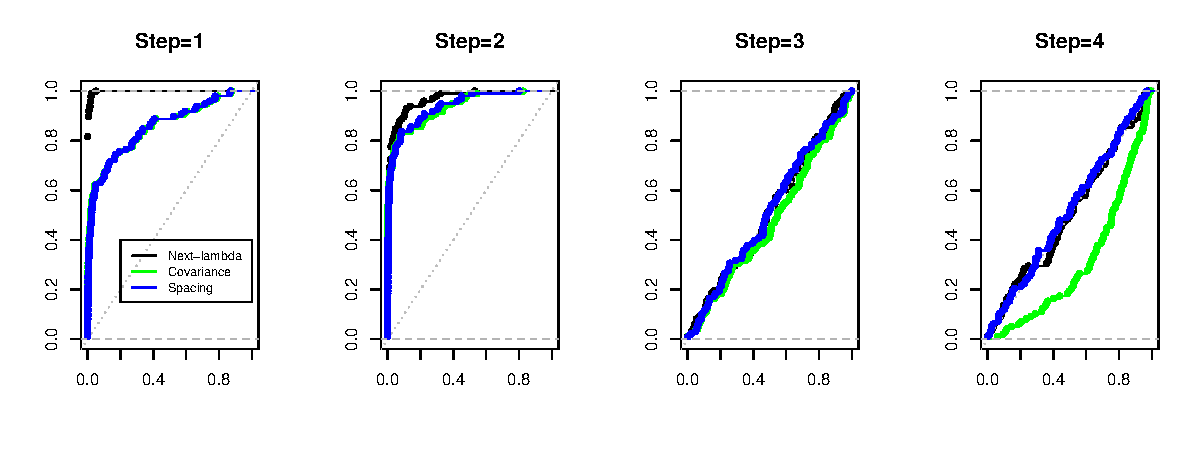
\includegraphics[width=\textwidth]{figs/larexample.pdf}
  \caption[fig:larexample]{\em  Cumulative distribution functions of $p$-values for LAR/lasso tests from simulations with $N=50,  p=10$ and two strong signals.}
  \label{fig:larexample}
\end{figure}

\subsection{Comparison of Selected- and Saturated-Model Inference}\label{sec:bivariate}

We now briefly compare the computational, conceptual, and statistical advantages and disadvantages of selected- and saturated-model tests, focusing on the problem of sequential model selection. For a detailed general discussion, see \citet[][Section 5]{fithian2014optimal}.

Selected-model inference is typically more computationally involved than saturated-model inference. Because the saturated-model test conditions on $n-1$ dimensions, the resulting distribution in~\eqref{eq:satModel} is nothing more than a truncated univariate Gaussian random variable. By contrast, selected-model tests typically require sampling from a truncated multivariate Gaussian distribution of dimension $p-|E_{k-1}|$.

For some applications, a major conceptual advantage of the saturated-model approach is that, when $M(E)$ is misspecified, $\theta^{E}$ is still a well-defined quantity on which we can perform exact inference. For example, a 95\% confidence interval for $\theta_{j_k}^{E_k}$ could cover that coefficient with probability 95\% even if $M(E_k)$ is misspecified. In the setting of sequential model selection, this advantage is less important: we are not looking for a scientifically interpretable interval for $\theta_{j_k}^{E_k}$; rather, the goal of the test at step $k$ is to reject $M_{k-1}$ and move on if it is demonstrably incompatible with the data. If there are many remaining strong signal variables to be found, then both $M_k$ and $M_{k-1}$ are badly misspecified; the more true this is, the stronger the grounds are for rejecting $M_{k-1}$.

\JTcomment{I would say our goal is a good stopping rule AND inference on parameters of selected (or perhaps saturated) model. We do not consider it here
because we don't know how to do it, not because it is not interesting.}

There are several major statistical benefits to selected-model inference. First, selected-model inference allows us to drop the assumption that $\sigma^2$ is known. This is not an option for the saturated model because conditioning on both $\|Y\|^2$ and $\proj_{\eta_k}^\perp Y$ results in a degenerate conditional distribution for $\eta_k'Y$.

Second, we have seen in Section~\ref{sec:pValsIndep} that tests of the form~\eqref{eq:selModel_cond} or~\eqref{eq:selModel_marg} yield independent $p$-values under general conditions, allowing us to apply  the sequential stopping rules of~\citet{gsell2013sequential} and \citet{li2015accumulation}.

Finally, and perhaps most importantly, selected-model tests can be dramatically more powerful than saturated-model tests, as we illustrate now with an extended example.

\begin{example}[Bivariate Regression with Identity Design]\label{ex:bivariate}
  Consider forward stepwise selection in a regression model with $n=p=2$, with known $\sigma^2=1$ and identity design 
\[
X = I_2=\begin{pmatrix} 1 & 0 \\ 0 & 1\end{pmatrix}.
\] 

The forward stepwise path and the lasso path both select $j_1=1$ if and only if $|Y_1|>|Y_2|$. The selection event $A_1=\{|Y_1| > |Y_2|\}$ is shown in yellow in Figure~\ref{fig:bv_condSets}. If $j_1=1$ then
\[
M_0:\; Y\sim \cN(0,I_2), \quad \text{ and } \quad
M_1:\; Y \sim \cN\left(\binom{\mu_1}{0}, \; I_2\right).
\]

The selected-model test at step 1 compares $Y_1$ to its distribution under $M_0$ conditional on $A_1$, a test of $H_0:\;\mu_1=0$ in model $M_1$.\footnote{In this very simple example, the max-$z$, max-$z$-identify, and next-$\lambda$ tests all coincide.} By contrast, the saturated-model test is a test of $H_0:\; \mu_1=0$ in the model $M_{\text{sat}}:\; Y \sim \cN(\mu, I_2)$. Thus, it must condition on $Y_2$ to eliminate the nuisance parameter $\mu_2$, comparing $Y_1$ to its null distribution given $A_1$ and the observed value of $Y_2$.

Figure~\ref{fig:bv_condSets} shows the conditioning sets for each model when $Y=(2.9, 2.5)$. Beside it, Figure~\ref{fig:bv_nullDists} shows the null conditional distribution of the test statistic $Y_1$ for each test. The $p$-values for the selected and saturated models are 0.007 and 0.3, respectively. These two plots are reproduced from \citet{fithian2014optimal}, in which the same example was presented in less detail.
\end{example}

\begin{figure}
  \centering
  \begin{subfigure}[t]{.4\textwidth}
    % source code: bivariateSelVSat.R
    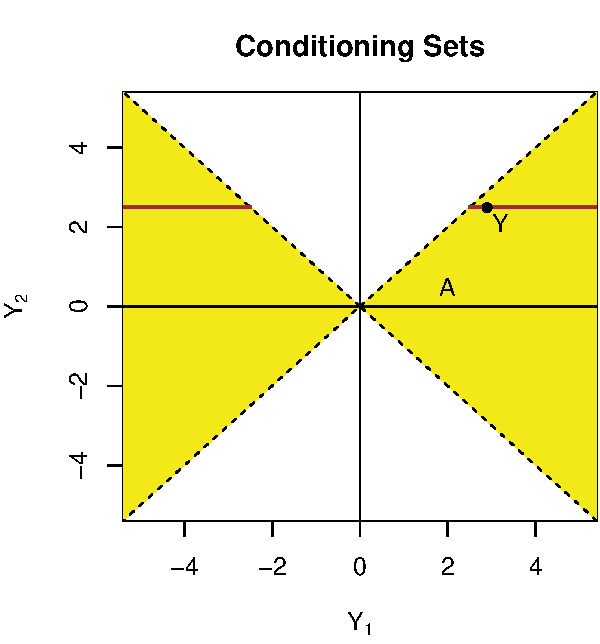
\includegraphics[width=\textwidth]{figs/bivariateSelVSat_condSets.pdf}
    \caption{The selected-model test conditions on $j_1=1$ (yellow region), while the saturated-model test also conditions on $Y_2=2.5$ to eliminate the nuisance variable $\mu_2$ (brown line segments).}
    \label{fig:bv_condSets}
  \end{subfigure}
  \hspace{.1\textwidth}
  \begin{subfigure}[t]{.4\textwidth}
    % source code: bivariateSelVSat.R
    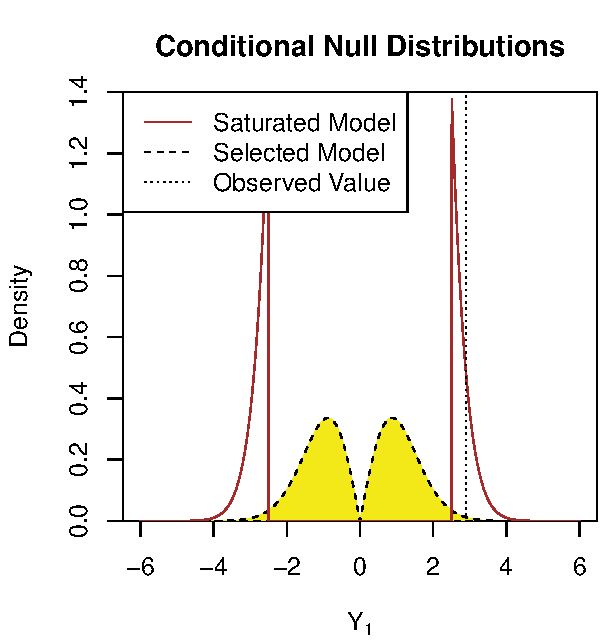
\includegraphics[width=\textwidth]{figs/bivariateSelVSat_nullDists.pdf}
    \caption{Conditional distributions of $Y_1$ under
      $M_0:\; Y \sim \cN(0,I_2)$. The realized value $|Y_1|=2.9$ is
      quite large given that $j_1=1$. By
      contrast, $|Y_1|=2.9$ is not especially large once we 
      also condition on $Y_2=2.5$.}
  \label{fig:bv_nullDists}
  \end{subfigure}
  \caption{Contrast between the saturated-model and selected-model
    tests in Example~\ref{ex:bivariate}. The selected-model test is based on  $\L(Y_1 \gv j_1=1)$,  whereas the saturated-model test is based on $\L(Y_1  \gv Y_2, \; j_1=1)$. 
    When $Y=(2.9, 2.5)$, the selected- and saturated-model $p$-values are 0.007 and 0.3, respectively.}
  \label{fig:bv}
\end{figure}

Figure~\ref{fig:bv} illustrates a general phenomenon in saturated-model tests: when there are near-ties between strong variables that are competing to enter the model, the resulting $p$-value my be very weak~\citep{lockhart2014significance}. Figure~\ref{fig:bv_rocCurve} displays the cumulative distribution function for the first $p$-value when $\mu=(4,4)$, a very strong signal. While the selected-model test has nearly perfect power, it is not uncommon for the saturated-model test to produce large $p$-values, even in the range of 0.5-0.9. These large $p$-values arise when there is a near tie between the variables.

\begin{figure}
  \centering
  % source code: bivariateSelVSat.R
  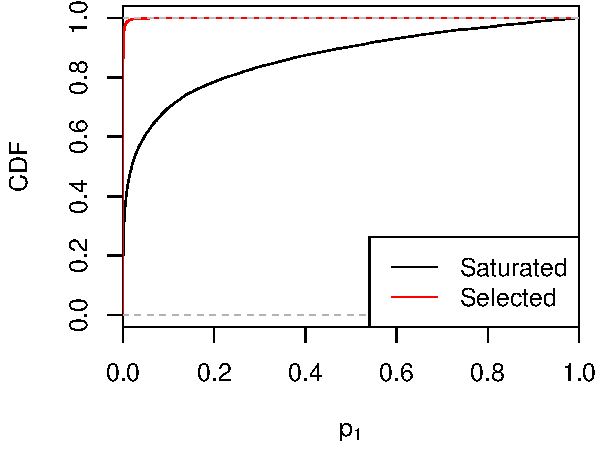
\includegraphics[width=.5\textwidth]{figs/bivariateSelVSat_rocCurve.pdf}
  \caption{Cumulative distribution function of $p_1(Y)$ for the selected- and saturated-model tests when $\mu=(4,4)$. Even though the signal is very strong, the saturated-model test results in large $p$-values in realizations like the one in Figure~\ref{fig:bv_nullDists}, where there is a near-tie between $|Y_1|$ and $|Y_2|$. By contrast, the selected-model test has nearly perfect power.}
  \label{fig:bv_rocCurve}
\end{figure}

Results in \citet{fithian2014optimal} show that the selected-model test is strictly more powerful when the selected model is correct; i.e., when $\mu_2=0$. Figure~\ref{fig:bv_powCurves} shows the power curve for each test when $\mu_2=0$ (left panel) and $\mu_2=4$ (right panel). While the selected-model test is more powerful when the selected model is correct, the difference between the two is relatively small. The difference is much more pronounced when $\mu_2=4$.

Note that if $\mu=(0,4)$, the incremental null is true, but the complete null is false. That is, the model $M_0 = M(\emptyset)$ is missing an important signal variable, but the missing variable is not $X_1 = (1,0)$. Because the saturated-model test is a valid test of the incremental null, its power is $\alpha=0.05$. By contrast, the selected-model test rejects about half of the time when $\mu=(0,4)$, detecting the fact that $M_0$ is a poor fit to the data.

\begin{figure}
  \centering
  \begin{subfigure}[t]{.4\textwidth}
    % source code: bivariateSelVSat.R
    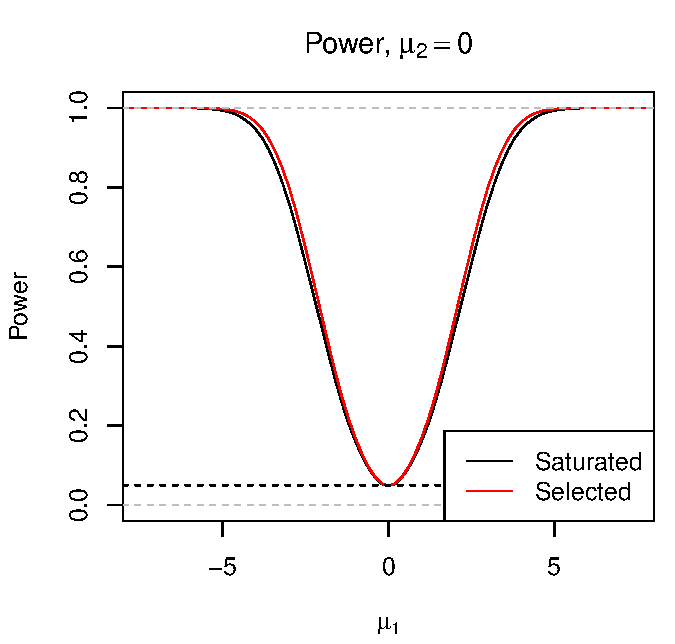
\includegraphics[width=\textwidth]{figs/bivariateSelVSat_powCurves_0.pdf}
    %\caption{\WFcomment{Write caption here.}}
    %\label{fig:bv_powCurves_0}
  \end{subfigure}
  \hspace{.1\textwidth}
  \begin{subfigure}[t]{.4\textwidth}
    % source code: bivariateSelVSat.R
    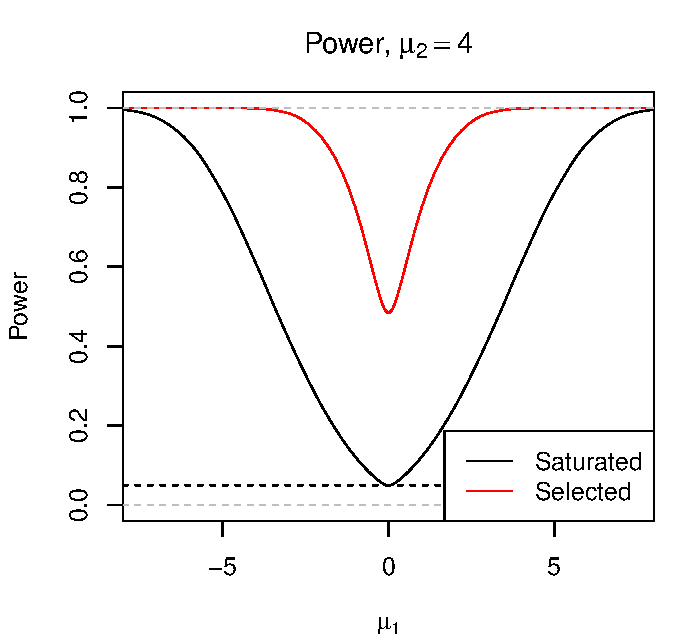
\includegraphics[width=\textwidth]{figs/bivariateSelVSat_powCurves_4.pdf}
    %\caption{\WFcomment{Write caption here.}}
  \end{subfigure}
  \caption{Power at level $\alpha=0.05$ for saturated- and selected-model tests at step 1, given that $j_1=1$. The power is plotted as a function of $\mu_1$, for two different values of $\mu_2$. When $\mu_2=0$, the selected-model test is strictly more powerful than the saturated-model test, but the difference is slight. By contrast, when $\mu_2=4$, the selected-model test is much more powerful. The dashed line shows $\alpha=0.05$.}
   \label{fig:bv_powCurves}
\end{figure}

Saturated-model $p$-values are generically non-independent. Continuing with Example~\ref{ex:bivariate}, Table~\ref{tab:bv_twoWayTable} shows a two-way contingency table for the saturated-model $p$-values $(p_1(Y), p_2(Y))$, binned into cells of height and width 0.2, simulated under the global null $\mu=0$. Because $k_0=0$, both $p$-values are uniform by construction, but the $p$-values are strongly dependent, with correlation $-0.48$. By contrast, the selected-model $p$-values $(p_1,p_2)$ are independent under the global null, a consequence of Theorem~\ref{thm:suffCond}.

\begin{comment}
Computing the cutoff for the saturated-model test requires us to know $\proj_{\eta}^\perp Y$, which is not $\sF_k$-measurable.

By contrast, selected-model tests of $M_{k-1}$ against $M_k$ are always $\sF_k$-measurable, because they are based on the law
\begin{equation}\label{eq:selModel}
\L\left(X_{j_k}'Y \mid X_{E_k-1}'Y, E_{k-1}, j_k\right),
\end{equation}
and all of the random variables appearing in~\eqref{eq:selModel} are $\sF_k$-measurable.
\end{comment}

% latex table generated in R 3.0.2 by xtable 1.7-1 package
% Mon May  4 21:11:15 2015
\begin{table}[ht]
  \centering
  \begin{tabular}{l|ccccc|c}
    \multicolumn{7}{c}{Saturated-Model $p$-Values 
      (\% of $10^6$ Simulations)}\\[7pt]
    \hline
    \multicolumn{7}{c}{}\\[-1.5ex]
    \multicolumn{7}{c}{$p_2(Y)$}\\[5pt]
    ${\large p_1(Y)}$ & (0,0.2] & (0.2,0.4] & (0.4,0.6] & (0.6,0.8] & (0.8,1] & \textbf{Total} \\ 
    \hline
    (0,0.2] & 1.0 & 2.7 & 4.2 & 5.6 & 6.7 & 20.1 \\ 
    (0.2,0.4] & 1.4 & 3.4 & 4.5 & 5.2 & 5.5 & 20.0 \\ 
    (0.4,0.6] & 2.3 & 4.3 & 4.7 & 4.5 & 4.2 & 20.0 \\ 
    (0.6,0.8] & 4.2 & 5.4 & 4.3 & 3.4 & 2.7 & 20.0 \\ 
    (0.8,1] & 11.1 & 4.3 & 2.3 & 1.4 & 1.0 & 20.0 \\ 
    \hline
    \textbf{Total} & 19.9 & 20.0 & 20.0 & 20.1 & 20.0 & 100.0 \\ 
    \hline
  \end{tabular}
  \caption{Two-way contingency table of saturated-model $p$-values $(p_1(Y), p_2(Y))$ for Example~\ref{ex:bivariate}, after binning into cells of height and width 0.2. We report the percentage of $p$-value pairs falling into each cell out of one million simulations from the global null hypothesis, $\mu=0$. Both $p$-values are marginally uniform but strongly dependent, with a correlation of $-0.48$.}
\label{tab:bv_twoWayTable}
\end{table}

\begin{comment}
First, note that $p_2$ is a selective $p$-value for comparing the null with only variable 1,
\[
M_1:\; Y \sim \cN\left(\binom{\mu_1}{0}, I_2\right),
\]
against the alternative with variables 1 and 2:
\[
M_2:\; Y \sim \cN\left(\mu, I_2\right), \text{ with } 
\mu_2 \neq 0.
\]
To eliminate the nuisance parameter $\mu_1$, the test conditions on $Y_1$. Thus, $p_2$ is uniform given $Y_1$ on $A$. Second, note that on $A$, $p_1$ is a function only of $Y_1$. Thus, $(p_1,p_2)$ are independent uniform variables given that variable 1 is chosen first. By a similar argument, they would also be independent uniforms if $Y_2$ were chosen first; thus, $(p_1, p_2)$ are marginally uniform under the global null.
\end{comment}

\section{Computation}
\label{sec:computation}

Until this point, we have deferred discussing the question of how to actually compute the rejection cutoffs for the max-$t$ test, next-$\lambda$ test, or any of the other tests we have discussed. In each case, we have a test that rejects when some test statistic $T_k$ is large compared to the law
\begin{equation}\label{eq:genDist}
\L(T_k \,\mid\, M_{k-1}, U_{k-1}),
\end{equation}
under the null hypothesis that $F\in M_{k-1}$. As such, we have reduced computation of the $p$-value at step $k$ to a sampling problem: if we can sample values of $Y$ from the law~\eqref{eq:genDist}, we can numerically approximate the $p$-value to whatever precision we desire.

Due to the generality in which we have posed the problem here, we cannot give a general prescription for how to carry out this sampling. Instead, we give details of our computational strategy here for one case, the max-$z$ test in forward stepwise regression with known $\sigma^2$.

Given a model $M_{k-1}$   we need to sample from 
\begin{eqnarray}
L(X'_jY \,|\, E_{k-1},X'_{E_{k-1}}Y)
\label{eqn:maxtsamp}
\end{eqnarray}
with $Y\sim N(\mu, I \cdot \sigma^2)$.
The current model fit is $\proj_{E_{k-1}} Y$ and it is easy to see that (\ref{eqn:maxtsamp})  is equivalent to sampling
\begin{eqnarray}
Y^*=\proj_{E_{k-1}} Y + (I- \proj_{E_{k-1}}) Z; \;Z\sim N(0,I\cdot\sigma^2)
\label{eq:boot}
\end{eqnarray}
and then conditioning on the event $E_{k-1}(Y^*)= E_k(Y)$ (a polyhedron).
In other words, we need to condition on data vectors  $Y^*$ that yields the same
sequence of variables and coefficient signs up to step $k-1$. This is the challenging aspect of this computation.

\JTcomment{We actually don't really need to condition on the signs
for the theory to go through. It is only so that sampling is feasible.}

Note that  (\ref{eq:boot})  has the form of  (conditional) parametric bootstrap sampling, but  with  a novel twist:  the bootstrap residuals are projected into the subspace
orthogonal to the current fit.  The typical justification for the bootstrap is asymptotic, relying on the convergence of the parameter estimates to the true parameters.
But something magical  occurs in the selective sampling scheme (\ref{eq:boot}): this  sampling fixes the value of $ X_{E_{k-1}}^Ty$ and this conditioning
removes the dependence on nuisance parameters.
Hence  (\ref{eq:boot}) yields the exact (non-asymptotic) conditional distributions and $p$-values.

Figure \ref{fig:comparison} shows an example with $n=100, p=20$ and one strong signal, computing the max-$t$ $p$-value at Step 3.
The ``exact'' answer  was determined from bootstrap sampling with $20,000$ replications.
The Figures show the bias, variance and MSE of the estimates from accept/reject and hit and run, using between 1000 and 8000 samples, averaged
over 10 different starting seeds.
\begin{figure}[htp]
\centering
  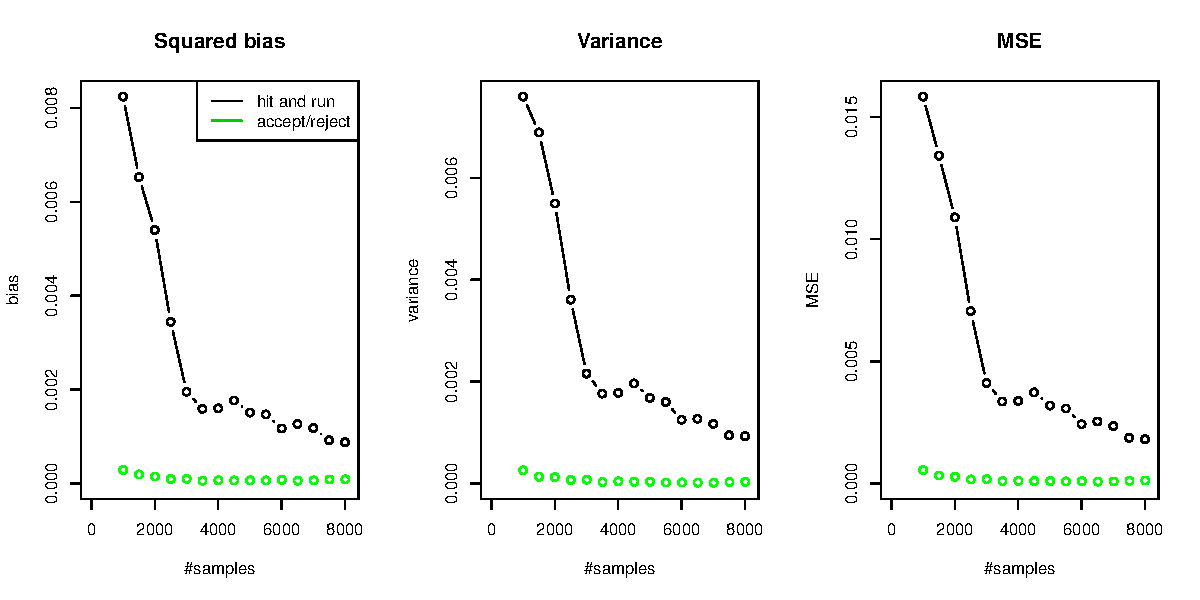
\includegraphics[width=\textwidth]{figs/comparison.pdf}
  \caption{\em Simulated example with $n= 100, p=20$ and one strong signal, computing the max-$t$ $p$-value at Step 3.  Shown are bias, variance and MSE of the estimates from accept/reject and hit and run, using between 1000 and 8000 samples, averaged
over 10 different starting seeds.
}
  \label{fig:comparison}
\end{figure}
We see that accept/reject is far more efficient, yielding a smaller MSE with 1000 samples then hit and run gives for  8000 samples.
Hence we use accept/reject for as many steps of the sequence is possible,  until the point where the acceptance rate is too low to make is practical.

In detail, we employ a hybrid computational strategy; we use accept-reject sampling, and do so as long as we obtain at least 300 (say) samples in the first set
of $B$ realizations ($75,000$ in our code)  This is an effective approach until we have reached a point in the model path where all predictors have little or no signal.
When the acceptance rate gets too low, we switch to a hit-and run Monte Carlo approach. We exploit the fact that each move along a random direction 
has a truncated Gaussian distribution whose truncation limits are easily computed from the properties of the polyhedron. Unlike accept-reject, sampling
which produces independent samples,  the hit and run method produces dependent samples. Hence we must run it for longer with an initial burn in period,
and hope that it has mixed sufficiently well.



The task is made much simpler by the fact that the selection event can we written as $S_M=\{y: \Gamma y \geq u\}$.
Hence we don't need to run the entire forward stepwise procedure on $y^*$: instead, we pre-compute $\Gamma$ and $u$ and then check
if $\Gamma y^* \geq u$. Further, since $\Gamma$ has on the  order of $2pk$ rows after $k$ steps,  we can save 
substantially in computation by checking the row-wise inequalities starting from the last row, where the inequality is most likely to fail.

\subsection{Reducing the number of constraints}
Happily, it turns out that the conditioning polytope can be expressed with only $2p$ constraints in forward stepwise regression, as we show here.
This increases the speed of both accept/reject and hit and Run sampling for our problem.

\begin{theorem}
  Assume the model path $M_{0:d}$ is obtained by forward stepwise 
  linear regression. Then, for a candidate active set $E$ of size $k$, 
  the set $A = \{E_k = E, \;X_E'Y = u\}$ is characterized 
  exactly by the constraints $X_E'Y=u$ and
  \[
  v_j^-(E,u) < X_j'Y < v_j^+(E,u), \quad\forall j \notin E,
  \]
  for $v_j^-$ and $v_j^+$ given explicitly in
  Equations~(\ref{eq:vMinus_FS}--\ref{eq:vPlus_FS}).
  Thus, $A$ corresponds exactly to 
  a set with $2(p-k)$ linear inequality constraints and $k$
  linear equality constraints on $Y$.
\end{theorem}

\begin{proof}
  At stage $i < k$, the next variable to enter is the one with maximal correlation with the residual vector; i.e.
  \[
  j_{i+1} = \argmax_{j \notin E_i} 
  \frac{\left| X_j ' (Y - X_{E_i}\hat\beta^i) \right|}
  {\|\proj_{E_i}^\perp X_j\|}
  \]
  The crucial observation is that, 
  once we know the $k$th active set 
  $E_k$ and its sufficient statistics
  $X_{E_k}'Y$, we know the entire 
  path of fitted models up to step $k$.
  On the set $\{E_k=E\}$, all of the quantities 
  $j_{i+1}$, $E_i$, $\hat\beta^i$, and $\proj_{E_i}^\perp$
  depend only on $X_E'Y$. For brevity, write
  \[
  C_i^* = \max_{j \notin E_i} 
  \frac{\left| X_j ' (Y - X_{E_i}\hat\beta^i) \right|}
  {\|\proj_{E_i}^\perp X_j\|}.
  \]
  On $A$, $C_i^*$ is attained at $j=j_{i+1}$, the $i$th 
  variable added.

  If $X_E'Y$ is fixed at $u$, and $j \notin E$, then the condition for 
  $X_j$ {\em not} to enter at step $i+1 < k$ is
  \[
  \frac{\left| X_j' (Y - X_{E_i}\hat\beta^i) \right|}
  {\|\proj_{E_i}^\perp X_j\|} 
  \leq C_i^*,
  \]
  or equivalently,
  \begin{equation}\label{eq:noEnterBounds_FS}
    X_j' X_{E_i}\hat\beta^i -
    C_i^*\|\proj_{E_{i}}^\perp X_{j}\|
    \;\;\;\leq\;\;\;
    X_j'Y
    \;\;\;\leq\;\;\;
    X_j' X_{E_i}\hat\beta^i +
    C_i^*\|\proj_{E_{i}}^\perp X_{j}\|, 
  \end{equation}
  so the set $A$ is equivalent to 
  Equation~\eqref{eq:noEnterBounds_FS} holding
  for every $i < k$ and $j \notin E$. Nominally, this gives $2k(p-k)$
  linear inequality constraints to satisfy, but most of them are
  non-binding. On $A$, the upper and lower bounds
  in~\eqref{eq:noEnterBounds_FS}
  are all known functions of $E$ and $u$, so we can set
  \begin{align}\label{eq:vMinus_FS}
    v_j^-(E,u) &= \max_{0 \leq i < k} \;\;X_j' X_{E_i}\hat\beta^i -
    C_i^*\|\proj_{E_{i}}^\perp X_{j}\| \\
    \label{eq:vPlus_FS}
    v_j^+(E,u) &= \min_{0 \leq i < k} \;\;X_j' X_{E_i}\hat\beta^i +
    C_i^*\|\proj_{E_{i}}^\perp X_{j}\|.
  \end{align}  
\end{proof}

As we see below, a similar result holds for the LASSO ever-active path. In fact, it holds for a much larger class of $\ell_1$-regularized exponential family models including the graphical LASSO.

\begin{theorem}
  Assume that $M_\infty$ is an exponential family model
  of the form
  \[
  Y \sim \exp\{ \theta'U(y) - \psi(\theta) \}\,d\nu(y),
  \]
  with $\Theta \sub \R^p$ convex, and assume
  that the model path $M_{0:d}$ is given 
  by the ever-active set for the $\ell_1$-penalized problem
  \begin{equation}\label{eq:regProblem}
  \hat\theta^r = \argmin_{\theta\in \Theta} 
  -\ell(\theta) + \lambda_r\|\theta\|_1,
  \end{equation}
  for some sequence $\lambda_r > 0$.

  Then, for a candidate active set $E$ of size $k$, 
  the set $A = \{E_k = E, \;U_E = u\}$ is characterized 
  exactly by the constraints $U_E = u$ and
  \[
  v_j^-(E,t) \leq U_j(Y) \leq v_j^+(E,t), \quad\forall j \notin E,
  \]
  for $v_j^-$ and $v_j^+$ given explicitly in
  Equations~(\ref{eq:vMinus_L1}--\ref{eq:vPlus_L1}).
  Thus, $A$ corresponds exactly to 
  a set with $2(p-k)$ linear inequality constraints and $k$
  linear equality constraints on $U(Y)$.
\end{theorem}

\JTcomment{Is there a reason you have $\psi$ and $\ell$ above instead of just $\ell$? I think the $(E,t)$ above should be $(E,u)$. It seems you never come back to $\psi$.}

\begin{proof}
  Note that, because exponential family likelihoods are concave in their natural parameters, the problem in~\eqref{eq:regProblem} is convex. Again, once we know the sufficient statistics $U_E(Y)$ for model $k$, and that $E_k=E$, we know that
  \[
  \hat\theta^r = \hat\theta^{(E,r)}
  \]
  for every $r \leq R_k$, so we know the entire path of fits up to and including $R_k$. But then, excluding variable $j \notin E$ at Lagrange parameter $\lambda_r$ is equivalent to
  \[
  \lambda_r \geq 
  \left| \pardd{\ell(\hat\theta^r)}{\theta_j} \right|
  = \left|U_j - \E_{\hat\theta^r}[U_j]\right|
  \]
  On $A$, for $r \leq R_k$, 
  $\E_{\hat\theta^r}[U_j]$ is a known function of $E$ and $u$,
  so we can set
  \begin{align}\label{eq:vMinus_L1}
    v_j^-(E,u) &= \sup_{r \leq R_k} \;\; 
    \E_{\hat\theta^r}[U_j] - \lambda_r \\
    \label{eq:vPlus_L1}
    v_j^+(E,u) &= \inf_{r \leq R_k} \;\;
    \E_{\hat\theta^r}[U_j] + \lambda_r .
  \end{align}
\end{proof}

\JTcomment{The notation $R_k$ isn't really defined. I don't think you need an
index $r$ and $k$, so we could talk about for every $\lambda \in \Lambda \geq \lambda_k$ instead of every $r \leq R_k$. No?
Here we do use the fact that the objective is a likelihood.}

\WFcomment{Give more general characterization of when we can do it, including group lasso? QP? Generalized Lasso?}

\begin{comment}
\subsection{An analytic approximation for the max-$t$ test}
 Suppose we have taken $k$ steps of forward stepwise regression with $p$ predictors and let the selected model  
 be $E$. Suppose we choose predictor $j^*$ at the next step.
 
Let $T_j=\eta_j^Ty, j \notin M$ be the partial regression coefficients for all predictors not in $E$,
and $(v_j^-, v_j^+)$ be the limits derived from the polyhedral lemma applied to $(E, \eta_j)$  (See e.g. \citet{spacings}).
These are the upper and lower bounds for the functional $\eta_j^Ty$ implied by the event that model $E$ is selected from the data $y$.
We chose the sign of $\eta_j$ so that $\eta_j^Ty$ is  $\geq 0$. 

 Let $F_{\mu,\sigma^2}^{a,b}(t)$ be the  cumulative distribution function of the truncated normal.
 Finally let $T=|T_{j^*}|$.
Then by assuming independence, a  simple approximation to the max-$t$ value is given by
\begin{equation}
1-\prod_{j\notin E} \{F_{0,||\eta||^2}^{v_j^-, v_j^+}(T)-   F_{0,||\eta||^2}^{v_j^-, v_j^+}(-T) \}
\label{eqn:approxpv}
\end{equation}
This approximation is exact if the predictors are uncorrelated.

Figure \ref{fig:approxpv} shows an example with $n=50$ and $p=10$ features having pairwise correlation 0.5.
There are two moderate signals.
Shown are the $p$-values from the ``exact'' numerical computation (with $100,000$ bootstrap samples)
and the approximation based on (\ref{eqn:approxpv}).
\begin{figure}[htp]
\centering
  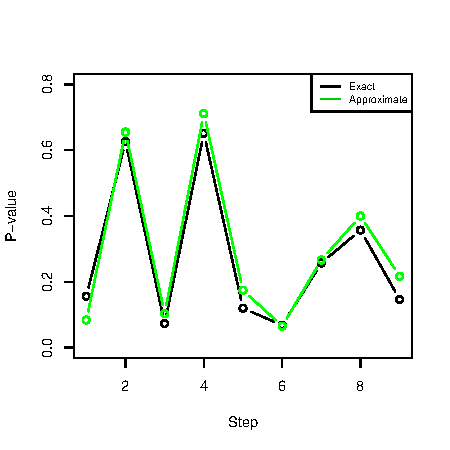
\includegraphics[width=3in]{figs/approxpv.pdf}
  \caption{Exact max-$t$ $p$-values and approximation based on (\ref{eqn:approxpv}), for a simulated example
  with $n=50, p=10$.}
  \label{fig:approxpv}
\end{figure}
The approximation seems quite good. By Sidak's lemma, we might conjecture that the approximation is conservative, but we have no proof of this.
\end{comment}

\section{Simulation: Sparse Linear Regression}
\label{sec:sparseReg}

Next we compare several model selection procedures in simulation. We simulate from a linear regression model with $n=100$ observations and $p=40$ variables. The design matrix $X\in\R^{n\times p}$ is a random Gaussian design with pairwise correlations of 0.3 between predictor variables.

The columns of $X$ are normalized to have length 1, and we simulate from $Y \sim \cN(X\beta,I_n)$, using a seven-sparse model with signal-to-noise ratio 5:
\[
\beta_j = \left\{\begin{matrix}5 & j = 1,\ldots,7\\ 0 &
    j>7\end{matrix}\right.
\]
We use known $\sigma^2=1$, so that we can compare the saturated-model test with the selected-model test. For our selection algorithm, we use the entire forward-stepwise path, for all 40 steps. 

\subsection{Single-Step $p$-Values}

For each step we compute one-step selected-model and saturated-model $p$-values, as well as nominal (unadjusted) $p$-values, conditioning on the signs of the active variables to make the problem more computationally tractable. Figure~\ref{fig:simulation_null_false} shows the power of all three tests for each of the first ten steps, conditional on the event that the null hypothesis is false. It is clear from Figure~\ref{fig:simulation_null_false} that the selected-model $p$-values are far more powerful than the saturated-model $p$-values. The nominal $p$-values are also quite powerful, but they do not have the correct level.

\begin{figure}[h]
  \centering
  % source code: ??? for simulation, sparseSim.R for plotting
  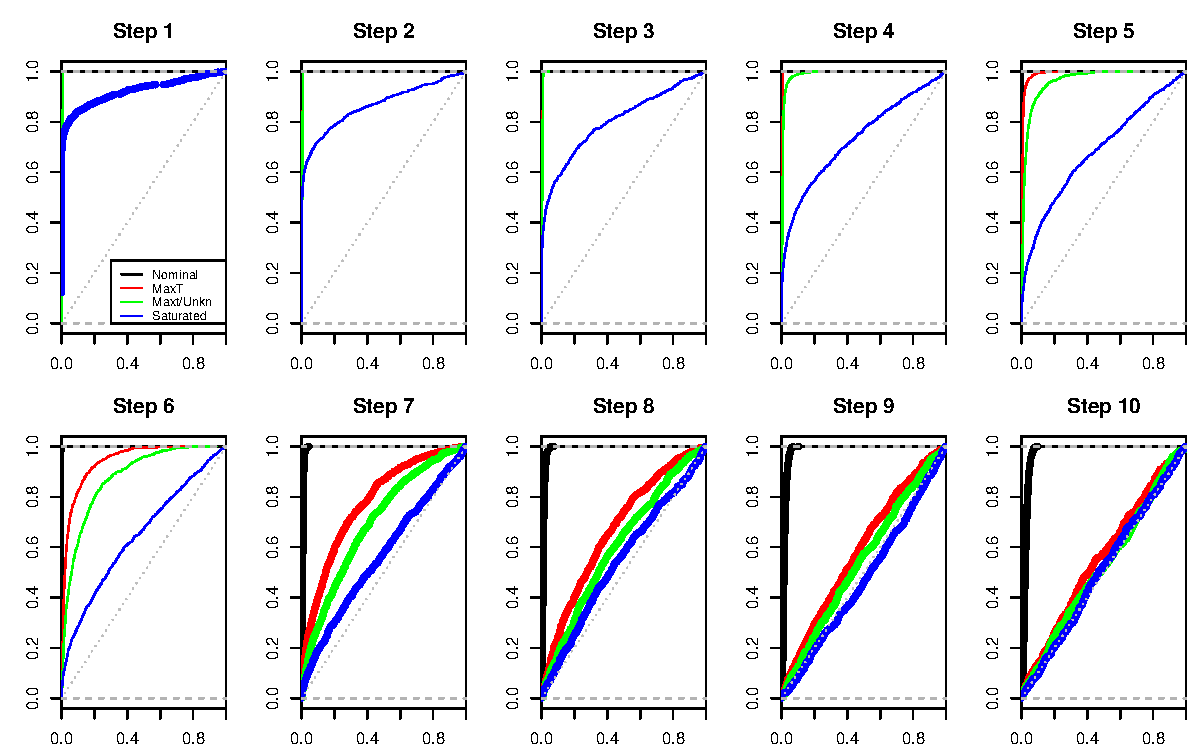
\includegraphics[width=1\textwidth]{figs/simulation_snr_5_alpha_05_null_false.pdf}
  \caption{\em  CDFs of nominal (black), MaxT (red), MaxT with unknown $\sigma$ (green) and  saturated-model (blue) $p$-values in the simulation of Section~\ref{sec:sparseReg}, conditional on testing a false null hypothesis at step $k$. The MaxT approaches are much more powerful than the saturated-model test. The nominal test appears to be powerful, 
  but is not $U(0,1)$ under the null, as shown below in Figure \ref{fig:simulation_null_true}.}
  \label{fig:simulation_null_false}
\end{figure}

\begin{figure}[h]
  \centering
  % source code: ??? for simulation, sparseSim.R for plotting
  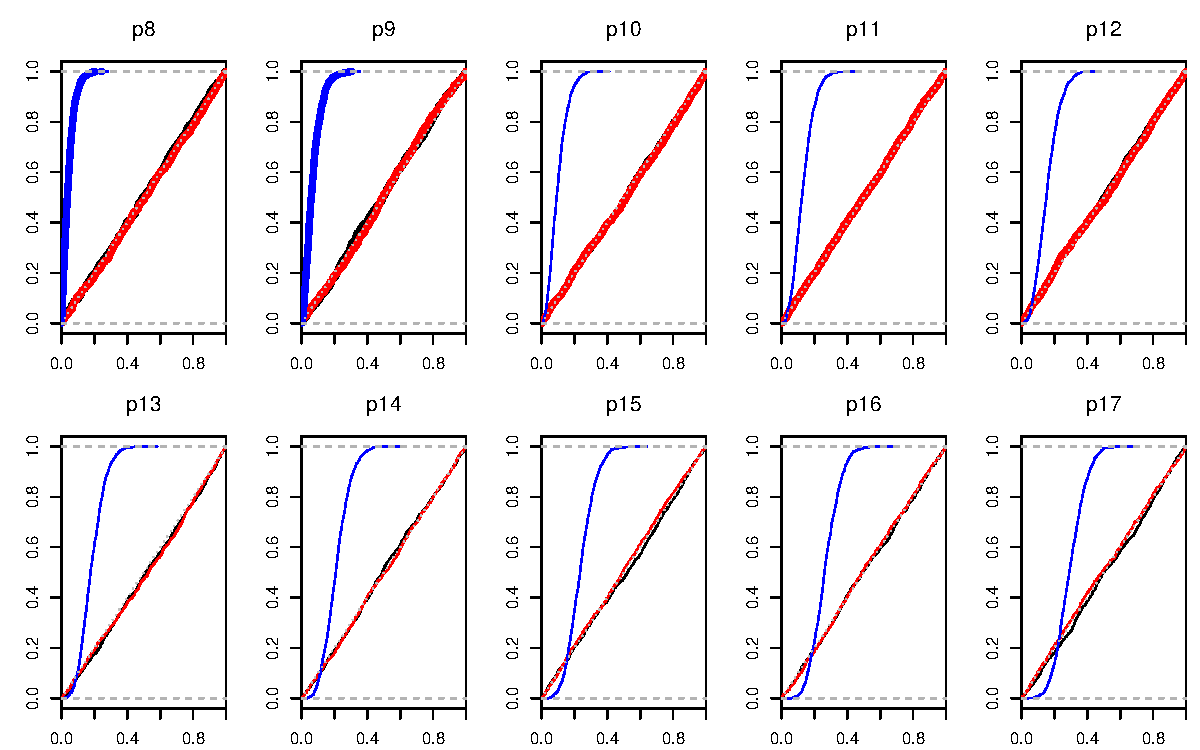
\includegraphics[width=1\textwidth]{figs/simulation_snr_5_alpha_05_null_true.pdf}
  \caption{\em  CDFs of nominal (black), MaxT (red), MaxT with unknown $\sigma$ (green) and  saturated-model (blue) $p$-values in the simulation of Section~\ref{sec:sparseReg}, conditional on testing a true null hypothesis at step $k$.  The nominal test is badly anti-conservative, while all of the other methods  show uniform $p$-values as desired.}
  \label{fig:simulation_null_true}
\end{figure}

\begin{figure}[h]
  \centering
  % source code: ??? for simulation, sparseSim.R for plotting
  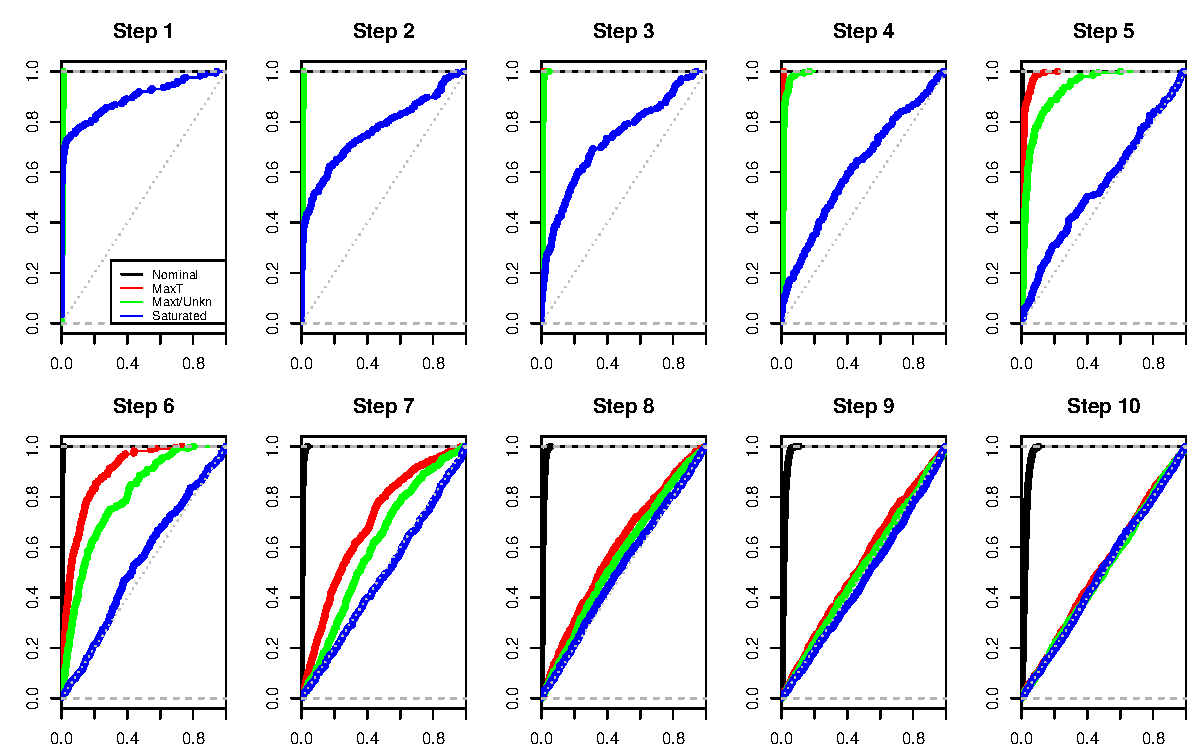
\includegraphics[width=1\textwidth]{figs/simulation_snr_5_alpha_05_noise_var.pdf}
  \caption{\em CDFs of nominal (black), MaxT (red), MaxT with unknown $\sigma$ (green) and  saturated-model (blue) $p$-values in the simulation of Section~\ref{sec:sparseReg}, conditional on the event that the variable added at step $k$ is a noise variable in the full model. Here, none of the methods produce uniform $p$-values. The null hypothesis is false in most cases and so --- in our model-centric point of view --- rejection is the desired outcome.}
  \label{fig:simulation_noise_var}
\end{figure}

Figure~\ref{fig:simulation_null_true} shows the distribution of $p_k$ for $k = 8, \ldots, 17$, given that the null hypothesis tested at step $k$ is correct (i.e., that $k_0< k$). Because the correct model is seven-sparse, $k=8$ is the first index for which the null can possibly be true. All but the nominal $p$-values are uniform by construction, but the nominal $p$-values are highly anti-conservative, as expected.

Finally, as a warning against misinterpretation of our method, we include Figure~\ref{fig:simulation_noise_var} showing the first ten $p$-values for each method, conditional on event that the variable added at step $k$ is a noise variable in the full model. Now, none of the $p$-values are uniform. 

This is not an error in our implementation of the method, but rather a consequence of our ``model-centric'' point of view. If we try to add a noise variable to the model before we have included all the signal variables, then we are testing a false null hypothesis. The test rejects because there is much more signal to find, and as such, it is entirely appropriate for us to reject the null and continue growing the model.

\subsection{Model-Selection Performance}

If we combine the saturated-model or selected-model $p$-values with one of our three stopping rules, we can evaluate the model-selection performance of each method in terms of:
\begin{itemize}
\item its probability of selecting a correct model or $p_{\text{screen}}$,
\item its model-wise FWER,
\item its model-wise FDR, and
\item its variable-wise FDR, where we use $V^{\text{full}}= \#\{\text{ noise variables included in } M_{\hk}\}$ instead of $V=(\hk-k_0)_+$.
\end{itemize} 
The last measure of performance is not explicitly controlled by any of the selective-inference methods, but we might nevertheless hope to perform reasonably.

% latex table generated in R 3.0.2 by xtable 1.7-1 package
% Fri May  1 09:29:28 2015
%\begin{table}[ht]
 % \centering
 % \begin{tabular}{llcccc}
  %  \hline
  %  Method & Stopping Rule & $p_{\text{screen}}$ & $\text{FWER}_{\text{mod}}$ an
 %   & $\text{FDR}_{\text{mod}}$ 
  %  & $\text{FDR}_{\text{var}}$ \\ 
 %   \hline
    %Selected & Basic & .290 & .000 & .002 & .039 \\ 
   % Selected & Forward & .559 & .027 & .020 & .066 \\ 
   % Selected & Strong & .041 & .014 & .008 & .042 \\ 
  %  \hline
   % Saturated & Basic & .000 & .000 & .000 & .028 \\ 
  %  Saturated & Forward & .014 & .000 & .000 & .030 \\ 
  %  Saturated & Strong & .000 & .000 & .000 & .032 \\ 
  %  \hline
  %  Knockoffs & & .000 & --- & --- & .231 \\ 
  %  \hline
 % \end{tabular}
 % \caption{\WFcomment{Comment on results once they are correct. These numbers are wrong right now.}}
%\end{table}

\begin{table}[ht]
\centering

\newcommand{\guarantee}[1]{{\color{blue} #1}}
\begin{tabular}{|l|rrrrrr|}
 \hline
{} &  $p_{\text{screen}}$ &  $\text{FWER}_{\text{mod}}$ &  $\text{FWER}_{\text{mod}} \vert \text{screen}$ &  $\text{FDR}_{\text{model}}$ &  $\text{FDR}_{\text{var}}$ &  $\text{S}_{\text{var}}$ \\ \hline
Nominal simple & 0.835 & 0.538 & 0.645 & 0.099 & 0.174 & 6.823 \\ 
Nominal forward & 0.931 & 0.918 & 0.985 & 0.348 & 0.430 & 6.927 \\ 
Nominal strong & 0.003 & 0.000 & 0.000 & 0.000 & 0.040 & 5.248 \\ 
MaxT simple & 0.364 & \guarantee{0.019} & \guarantee{0.052} & \guarantee{0.002} & 0.047 & 6.124 \\ 
MaxT forward & 0.675 & 0.190 & 0.281 & \guarantee{0.028} & 0.086 & 6.605 \\ 
MaxT strong & 0.027 & \guarantee{0.006} & 0.229 & \guarantee{0.003} & 0.038 & 4.829 \\ 
MaxT identify simple & 0.398 & \guarantee{0.023} & \guarantee{0.057} & \guarantee{0.003} & 0.047 & 6.175 \\ 
MaxT identify forward & 0.694 & 0.189 & 0.272 & \guarantee{0.028} & 0.086 & 6.641 \\ 
MaxT identify strong & 0.021 & \guarantee{0.006} & 0.286 & \guarantee{0.003} & 0.041 & 4.856 \\ 
MaxT unknown simple & 0.312 & \guarantee{0.019} & \guarantee{0.061} & \guarantee{0.002} & 0.046 & 5.927 \\ 
MaxT unknown forward & 0.638 & 0.168 & 0.264 & \guarantee{0.024} & 0.078 & 6.531 \\ 
MaxT unknown strong & 0.035 & \guarantee{0.005} & 0.152 & \guarantee{0.002} & 0.038 & 4.486 \\ 
Saturated simple & 0.002 & 0.000 & 0.000 & 0.000 & 0.033 & 1.802 \\ 
Saturated forward & 0.014 & 0.001 & 0.056 & 0.000 & 0.030 & 2.310 \\ 
Saturated strong & 0.000 & 0.000 & NA & 0.000 & 0.036 & 2.171 \\ 
Knockoff & 0.301 & NA & NA & NA & 0.106 & 4.306 \\ 
Knockoff+ & 0.000 & NA & NA & NA & \guarantee{0.000} & 0.000 \\   \hline
\end{tabular}
\caption[tab:stopping]{\em Results of various stopping rules applied to simulated data with 7 strong signals,  as described at the beginning of Section \ref{sec:sparseReg}.
The {\tt Simple} rule stops at the first time that a $p$-value exceeds $\alpha=0.05$, while {\tt Forward} and {\tt Strong} refers to the ForwardStop and StrongStrop rules of Section \ref{sec:orderedProposals}. Results with theoretical guarantees are \guarantee{highlighted}.}
\label{tab:stopping05}
\end{table}

\begin{table}[ht]
\centering

\newcommand{\guarantee}[1]{{\bf #1}}
{\small 
\begin{tabular}{|l l|cccccc|}
\hline
{} & {} &  $\P(\hk \geq k_0)$ &  $\text{FWER}$ &  $\text{cFWER}$ &  $\text{FDR}$ &  $\text{FDR}^{\text{full}}$ &  $\E[S^{\text{full}}]$ \\ \hline
Nominal & BasicStop & 0.94 & 0.93 & 0.99 & 0.415 & 0.498 & 6.94 \\ 
Nominal & ForwardStop & 0.98 & 0.98 & 1.00 & 0.640 & 0.704 & 6.98 \\ 
Max-z & BasicStop & 0.61 & \guarantee{0.12} & \guarantee{0.20} & \guarantee{0.018} & 0.073 & 6.53 \\ 
Max-z & ForwardStop & 0.86 & 0.64 & 0.75 & \guarantee{0.152} & 0.231 & 6.84 \\ 
Max-t & BasicStop & 0.58 & \guarantee{0.11} & \guarantee{0.19} & \guarantee{0.016} & 0.069 & 6.46 \\ 
Max-t & ForwardStop & 0.84 & 0.62 & 0.73 & \guarantee{0.140} & 0.219 & 6.82 \\ 
Saturated & BasicStop & 0.06 & 0.01 & 0.13 & 0.001 & 0.031 & 3.13 \\ 
Saturated & ForwardStop & 0.39 & 0.17 & 0.44 & 0.028 & 0.074 & 4.98 \\ 
Knockoff & & 0.59 & --- & --- & --- & 0.230 & 5.72 \\ 
Knockoff+ & & 0.36 & --- & --- & --- & \guarantee{0.136} & 3.76 \\  \hline
\end{tabular}}
\caption[tab:stopping]{\em Results of various stopping rules applied to simulated data with 7 strong signals,  as described at the beginning of Section \ref{sec:sparseReg}.
The {\tt Simple} rule stops at the first time that a $p$-value exceeds $\alpha=0.2$, while {\tt Forward} and {\tt Strong} refers to the ForwardStop and StrongStrop rules of Section \ref{sec:orderedProposals}. Results with theoretical guarantees are \guarantee{highlighted}.}
\label{tab:stopping20}
\end{table}

We see that 1) strongStop and forwardStop control FWER and modelwise FDR, respectively, using $p$-values from MaxT or MaxT-identify, as predicted by theory
2) the nominal $p$-values do not lead to control of FWER or FDR, as expected, 3) the $p$-values from the saturated model show FWER and modelwise-FDR control,
although not guaranteed by theory, 4) the MaxT rules show higher probabilities of selecting the true model, especially using forwardStop, 5) the knockoff method
does not yields variable-wise FDR control, as it should.
5)
\section{Principal Components Analysis}
\label{sec:pca}

\WFcomment{Can we do this one?}
\JTcomment{In principle, we can. But, paper is a little long. Maybe
just point out in discussion
that the $p$-values in Choi et al. are examples of this setup? The notation in Yunjin's paper is nothing like this, but we do form selected model tests with the sufficient statistic growing in dimension as we go down the path. In this case, ``maxT'' is the same as ``maxT identify'' where we ``identify'' the sets of singular vectors...}

Here we consider model selection for principal components analysis. In that case we are given a data matrix $X \in \R^{n\times d}$, with which we form a sample %covariance matrix
\[
S = \frac{1}{n-1} \sum_{i=1}^n(x_i - \bar x)^2
\]
The first $d$ principal component loadings are the first $d$ eigenvectors of $S$, which call $u_1,\ldots, u_d$. These induce a sequence of nested Wishart models:
\[
M_0 \sub M_1 \sub \cdots \sub M_d
\]
in which
\begin{equation}
  M_k:\; (n-1) S \sim W_d\left(\lambda_0 I_d + \sum_{i=1}^k     \lambda_i u_i u_i', \;\;\; n-1\right).
\end{equation}
 By successively conditioning on $u_j, j<k$ one can obtain an exact sequential test
for the complete null hypothesis $H_0: \lambda_j=0 \; \forall j \neq k$.  The computation of the resulting $p$-values requires numerical integration.
The details are given in \citet{choi2014selecting}, with their ``integrated CSV'' test  corresponding to the sequential selective test of this paper.

\RTcomment{Jon- add more details?}

\section{Decision trees and interaction models}
In this section we discuss another application of adaptive sequential inference, to binary decision trees.
Specifically, the classification and regression tree  (CART)  method builds a decision tree in a top down manner, finding the best available split
at each node.  When considering splitting two daughter nodes, the generic CART algorithm splits the nodes in an arbitrary order, only stopping when a node
reaches a minimum size.  We instead consider a  special version of CART  algorithm:  the   "best first"  method, which order splits by their achieved reduction in loss.
This procedure is used, for example in the R package for gradient boosting, called {\tt gbm}.
The best first tree-builder is thus a sequential selection  procedure,  to which we can apply the results in this paper. Hence we can obtain independent, sequential $p$-values
for each successive split in the decision  tree. We now give some details and an example.

Given data $(y_i, x_{i1}, x_{i2},\ldots x_{ip})$ for $i=1,2,\ldots N$,
we choose a splitting  variable $j_1$ and split point $t_1$, leading to a model of the form
\begin{eqnarray}
\hat y_i=\beta_0 +\beta_{11} I(x_{ij_1} \leq t_1) +\beta_{12} I(x_{ij_1} > t_1)
\end{eqnarray}
Then at the second stage, we try splitting one of the two daughter nodes, and choose the split and most reduces the residual sum of squares.
Suppose that a split of the first node is chosen, using predictor $j_2$ at split point $t_2$.  This leads to the interaction model of the form
\begin{eqnarray}
\hat y_i=\beta_0 +\beta_{11} I(x_{ij_1} \leq t_1) \cdot \beta_{31} I(x_{ij_2} \leq t_2)+   \beta_{11} I(x_{ij_1} \leq t_1) \cdot  \beta_{31} I(x_{ij_2} > t_2)  +\beta_{12} I(x_{ij_1} > t_1).\cr
\label{eqn:intmodel}
\end{eqnarray}
Note that the search for possible split points can be expressed through an exhaustive set of basis functions $I(x_{ij} \leq  t_i), I(x_{ij}  > t_i)$ for each $t_i \in (x_{1j}, x_{2j}, \ldots x_{nj})$.
The procedure is somewhat similar to foreward stepwise regression, but with differences.
For example the set of candidate basis functions available at each stage are a function of what has been  previously entered into the model
Nonetheless,  the selection procedure  for the first set of $k$ splits can be expressed in polyhedral from $Ay \leq b$, and the saturated and selective inference procedures can be applied.
As before, the saturated $p$-values have an explicit truncated Gaussian form, while computation of the selective $p$-values require accept-reject sampling.

Figure \ref{fig:cart} shows an example with independent standard Gaussian features, and $n=30, p=3$.
We 
consider just the first two splits, in a null case (top row) and non-null (bottom row).
In the non-null case,  the data are generated from a  model of the form (\ref{eqn:intmodel}).

As expect, the nominal $p$-values are far too small and hence don't control type I error.
Both the saturated and selective $p$-values control type I error, with the selective $p$-values are somewhat more powerful in the non-null case.
Rules like the forwardStop procedure could be applied  to the selective $p$-values to choose a ``best'' model size.
\begin{figure}[h]
  \centering
  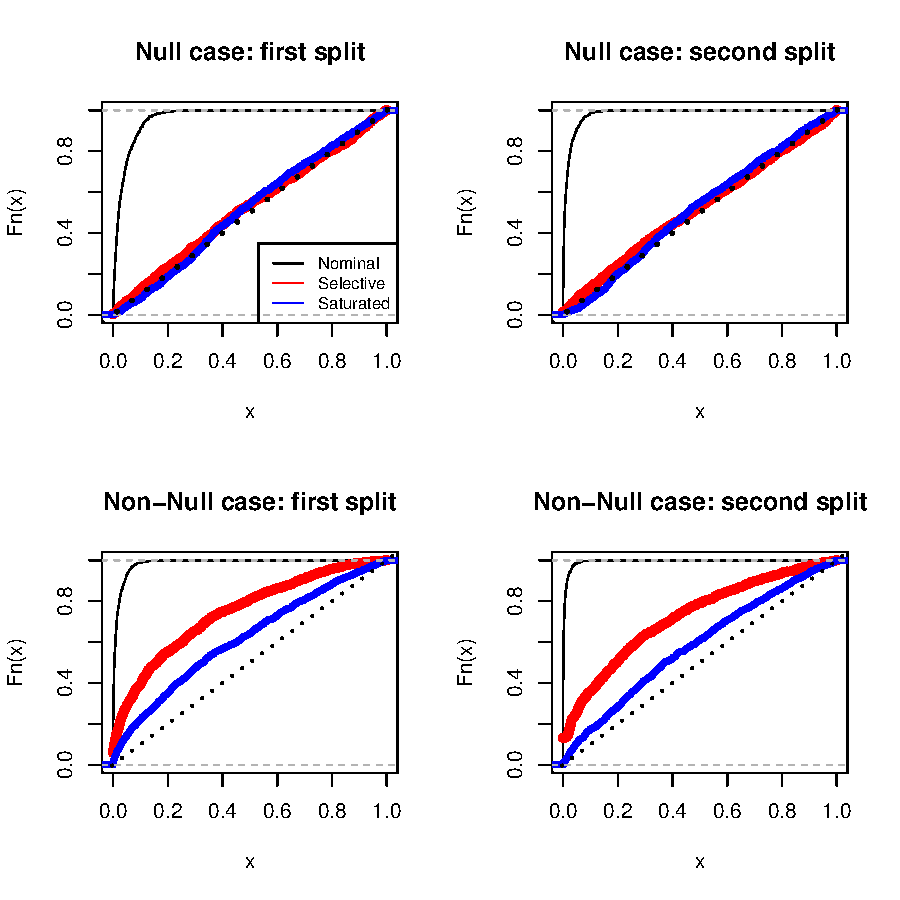
\includegraphics[width=.65\textwidth]{figs/cart.pdf}
  \caption{\em Cumulative distribution functions of $p$-values for  the first two splits in a CART decision tree. In the top row, the true model is null,
  while in the bottom row, the data are generated from a  model of the form (\ref{eqn:intmodel})}
  \label{fig:cart}
\end{figure}

\section{Discussion}
\label{sec:discussion}

\WFcomment{Adding variables in groups? Changing the set of variables to select from at each step?}

It is a commonplace that ``essentially all models are wrong, but some are useful'' \citep{box1987empirical}. In essence, a statistical model is useful if it is large enough to capture the most important features of the data, but still small enough that inference procedures can achieve adequate power and precision. Apart from theoretical considerations, the only way to know whether a model is large enough is to test whether it is, using available data.

Although model-checking is commonly recommended to practitioners as an important step in data analysis, it formally invalidates any inferences that are performed with respect to the model selected. Our work takes a step in the direction of reconciling that contradiction, but there are important questions left to be resolved. In particular: which sorts of model misspecification pose the most threat to our inferential conclusions, and how powerful are our tests against these most troublesome sources of misspecification? 

Of course, the answer depends on the scientific context: for example, suppose that at step 1, forward stepwise regression selects a variable $X_1$, and then at some later step it selects another variable $X_2$, which is almost perfectly correlated with $X_1$. There may be little evidence to support adding $X_2$ to the model once $X_1$ is already included, even if including $X_2$ would greatly change our inference about the coefficient for $X_1$ (for example, by making its confidence interval much wider). Depending on the context, we could draw the conclusion that 1) $X_1$ and $X_2$ are near-duplicate variables and it is therefore unnecessary (and possibly counterproductive) to include both in the model, or 2) $X_2$ is a vital confounding variable for $X_1$ and the confidence interval for $\beta_1$ ought to reflect the resultant uncertainty. If the second interpretation is the scientifically appropriate one, then we should probably use a different selection algorithm --- for example, a variant of forward stepwise that always adds both $X_1$ and $X_2$ to the model as a group in the same step.

We plan to distribute  open source software, in both the R and Python languages,  for computing the max-$t$ and other tests discussed in this paper.

\JTcomment{Max $T$ available in python code on github. I suppose R as well, but not sure.}

\section*{Acknowledgments}

The authors are grateful for stimulating and informative conversations with Stefan Wager, Lucas Janson, Trevor Hastie, ....

\bibliographystyle{plainnat}
\bibliography{biblio}

\end{document}


\begin{comment}
Sections~\ref{sec:pvalSP}--\ref{sec:modelSSP} discuss sufficient conditions on the $p$-values and the selection algorithm under which single-step $p$-values are automatically independent. Section~\ref{sec:selectionVariables} discusses how we can create independent $p$-values by conditioning on finer selection variables at each step.

Essentially, we will want to partition the information in $Y$ according to the filtration:
\begin{align}\nonumber
  \sF(M_0,T_0) &\underlabel_{\text{selection } 1} 
  \sF(M_{0:1},T_0) \underlabel_{\text{inference } 1}
  \sF(M_{0:1},T_1) \quad \sub \;\;\cdots\\[8pt]
  \label{eq:infoPartition}
  \cdots\;\; \sub \quad&
  \sF(M_{0:d-1},T_{d-1}) \underlabel_{\text{selection } d}
  \sF(M_{0:d},T_{d-1}) 
  \underlabel_{\text{inference } d}
  \sF(M_{0:d}, T_d)
\end{align}

\end{comment}

\begin{comment}
\WFcomment{There is a filtration interpretation when you have the appropriate sufficiency properties.} Let $\sF_{k,i}$ denote the $\sigma$-algebra generated by $M_{0:k}$ and $p_{1:i}$.
\begin{align*}
  \sF_{k,i} &= \sF(M_{0:k},p_{1:i})\\
  \sF_0 &\underlabel_{\text{selection } 1} \sF_{1,0} \underlabel_{\text{inference } 1}
  \sF_{1,1} \;\;\sub \cdots \sub\;\;
  \sF_{d-1,d-1} \underlabel_{\text{selection } d} \sF_{d,d-1}
  \underlabel_{\text{inference } d} \sF_{d,d}
\end{align*}
\end{comment}
